\documentclass[HardwareDesign/HardwareDesign_main.tex]{subfiles}
\begin{document}
\section{Cup Sensor} \label{sec:CupSensor}
I dette afsnit beskrives udviklingen af en sensor, Cup Sensor. Der designes både delen der skal være på i Cup Sensor blokken, Cup Holder Controller og på PSoC. Sensoren skal registrere når en kop placeres på en bestemt placering på bordet der udvikles i dette projekt. Sensoren skal hvis muligt også detektere når en bold rammer i koppen (er 
'should' i MoSCoW analysen). Dette kan gøres på flere forskellige måder som undersøges i det følgende underafsnit. Derudover skal der laves noget hardware der gør det muligt at få data fra 6 sensorer 'samtidig' (en del af Cup Holder Controller blokken)

\subsection{Teknologiundersøgelse} \label{sec:CupSensorTekUnder}
For at detektere en kop der er placeret, skal koppen med øl påvirke nogle fysiske egenskaber for en sensor, som dermed kan detekteres. Der overvejes forskellige egenskaber som kan detekteres, som kan ses i listen nedenfor. De forskellige punkter gennemgås detaljeret bagefter.
\begin{enumerate}
    \item \label{itm:cupSensor_weight} Kraft.
    \item \label{itm:cupSensor_lightReflection} Lys refleksion. 
    \item \label{itm:cupSensor_lightAbsorbtion} Lys absorption.
    \item \label{itm:cupSensor_capacitive} Dielektrikum.
\end{enumerate}

En kop med øl vil have en større masse end den luft den erstatter, derfor vil den overflade koppen står på blive udsat for en større kraft end før. Denne ændring kan dermed detekteres. En helt simpel metode vil være vha. en kontakt. Dette kan dog ikke bruges til at detektere at en bold rammer i koppen. En bold i koppen vil øge den samlede masse af koppen. En bold vil dog ikke veje så meget sammenlignet med en kop med øl. En bold i bevægelse der lander i koppen vil dog blive udsat for en kraft i det den skal deaccelereres, den overflade koppen står på vil derfor blive udsat for den samme kraft i modsat retning. Hvis der derfor laves en vægt-/kraftsensor kan denne muligvis detektere både placering af kop, men også detektere at en bold rammer i. Begge disse metoder vil kræve en bevægelse af den overflade som koppen står på. Det er et krav til at systemet skal være vandtæt,  dette er svært at overholde hvis der er ting som skal bevæge sig. Det vil sikkert være muligt, men formålet med dette projekt er ikke at arbejde med materialer mm.

Grundet problemet med at holde systemet vandtæt, overvejes nu kun metoder som kan "se"  igennem bordoverfladen. En kop reflekterer lys. Dette kan derfor være muligt at sende lys op gennem en gennemsigtigt bordoverflade, og måle på det lys der reflekteres tilbage. Dette kræver en gennemsigtig bordoverflade. Derudover vil det måske være muligt at detektere at en bold rammer i da der vil reflekteres mere lys når bolden er der.

En kop, både gennemsigtig og ikke gennemsigtig, vil absorbere/blokere for lys. Dette kan bruges på forskellige måder. Fx kan der måles på det lys som modtages fra omgivende lys. Hvis der bliver placeret en kop som dermed blokerer for/absorberer dette lys, kan det detekteres. Denne metode vil dog være afhængig af den omgivende lys, og det kan variere meget da systemet kan blive brugt i meget lyse omgivelser og i meget mørke omgivelser. Dette er derfor ikke så god en metode. En anden metode der bruger en kops absorbtionsegenskaber er at sende lys i den ene side af en kop og måle på den anden side.  Denne metode er dog ikke så elegant da det enten vil kræve neddybninger i bordet til kopperne eller at sensoren stikker op fra bordet. Begge disse situationer ønskes ikke, da der ønskes en flad bordoverflade.

En kop med øl, vil have en anden dielektrikum end luften. Derfor kan der laves en kapacitiv sensor som måler kapaciteten (som er afhængig af dieletrikum) som påvirkes af materialet omkring kop sensoren (vil blive forklaret mere i detalje). Denne metode har den fordel at man kan "se" igennem bordet, så længe overfladen har en relativ lav dielektricitetskonstant.

Der er, som beskrevet, nogle metoder hvor der er åbenlyse ulempe som vælges fra med det samme. Der vælges to metoder som undersøges nærmere: lys reflektion og dielektrikum. Disse metoder undersøges til sådan en grad så det er muligt at træffe et valg mellem de to metoder (eller fravælge dem begge og finde en ny metode). Teknologiundersøgelserne bliver hermed brugt til en form for 'proof of concept'.  

\subsubsection{Kapacitiv sensor}
Til at måle en ændring i dielektricitetskonstanten, benyttes en kapacitiv sensor. Fra den første EFYS øvelse, blev det vist at man kan male den frie kapacitet af en metalplade. Den kapacitet som måles er kapaciteten mellem pladen og en sfærisk overflade uendelig langt væk. I realiteten er det bare en stel forbindelse som er tilstrækkelig nok væk. Når der placeres en kop med øl vil der være en større dielektricitetskonstant som dermed øger den frie kapacitet. Det kan betragtes som at pladens areal nu forøges til arealet af overfladen af væsken. Der overvejes også en metode hvor der benyttes to plader, hvor der måles kapaciteten mellem de to plader.

Til at måle kapaciteten af en så relativ lille kondensator kan der benyttes CapSense på PSoC'en. Her skal der ikke benyttes noget ekstra hardware end det der allerede er i PSoC'en (selve microcontrolleren) samt en kondensator som Cypress kalder $C_{MOD}$ med værdien 2.2nF for en PSoC 5LP \autocite[115]{AN64846}. Den er allerede på udviklingskittet på ben P15[4] \autocite[2]{PSoCKitSchematics}. Til CapSense er der knyttet en del automatisk signal behandling. En funktionallitet der er i CapSense er at den benytter hvad de kalder en 'baseline'\autocite[18]{AN64846}. Denne baseline er den læste værdi når der ikke er en kop, eller andre ting der skal måles med CapSense. Nyttesignalet beregnes ud fra baseline så signalet er 0 (eller tæt på) når der ikke er en kop. Denne baseline kan ændre sig som omgivelserne ændre sig, fx temperaturændring. Der benyttes et lavpasfilter til at opdatere baseline, så længe den holder sig inden for en given 'noise threshold', ellers betragtes det som et nyttesignal.

Der laves først en ikke dokumenteret test hvor der undersøges de to forskellige metoder som tidligere beskrevet. Den ene er hvor den frie kapacitet måles, den anden er hvor der benyttes to plader. Til den frie kapacitet bruges en kopperplade på ca 30mmx33mm. Til den med to plader benyttes den samme plade, men med en ledning rund om den som fungere som den anden plade. Der observeres ikke nogen synlig forskel i signalet mellem de to metoder, derfor fortsættes nu kun med den frikapacitet.

Der benyttes testopstillingen som det ses på figur \ref{fig:cap_tape_testopstilling} og figur \ref{fig:cap_testopstilling}. 
Der laves forskellige test. Test hvor der placeres en kop med øl og fjernes igen. Test hvor der placeres en øl og der slippes en bold som falder ned i koppen. Det testes hvad indflydelsen af en hånd på toppen af koppen har. Der testes også med ca 110ml øl og 220ml øl. Til at få dataen fra CapSense benyttes PSoC'ens CapSense Tuner program. Målingerne kan ses på figur \ref{fig:cap_test_place_and_remove_110}, \ref{fig:cap_test_place_and_hand_110}, \ref{fig:cap_test_place_and_drop_110}, \ref{fig:cap_test_place_and_remove_220} og \ref{fig:cap_test_place_and_drop_220}


\begin{figure}[H]
    \centering
    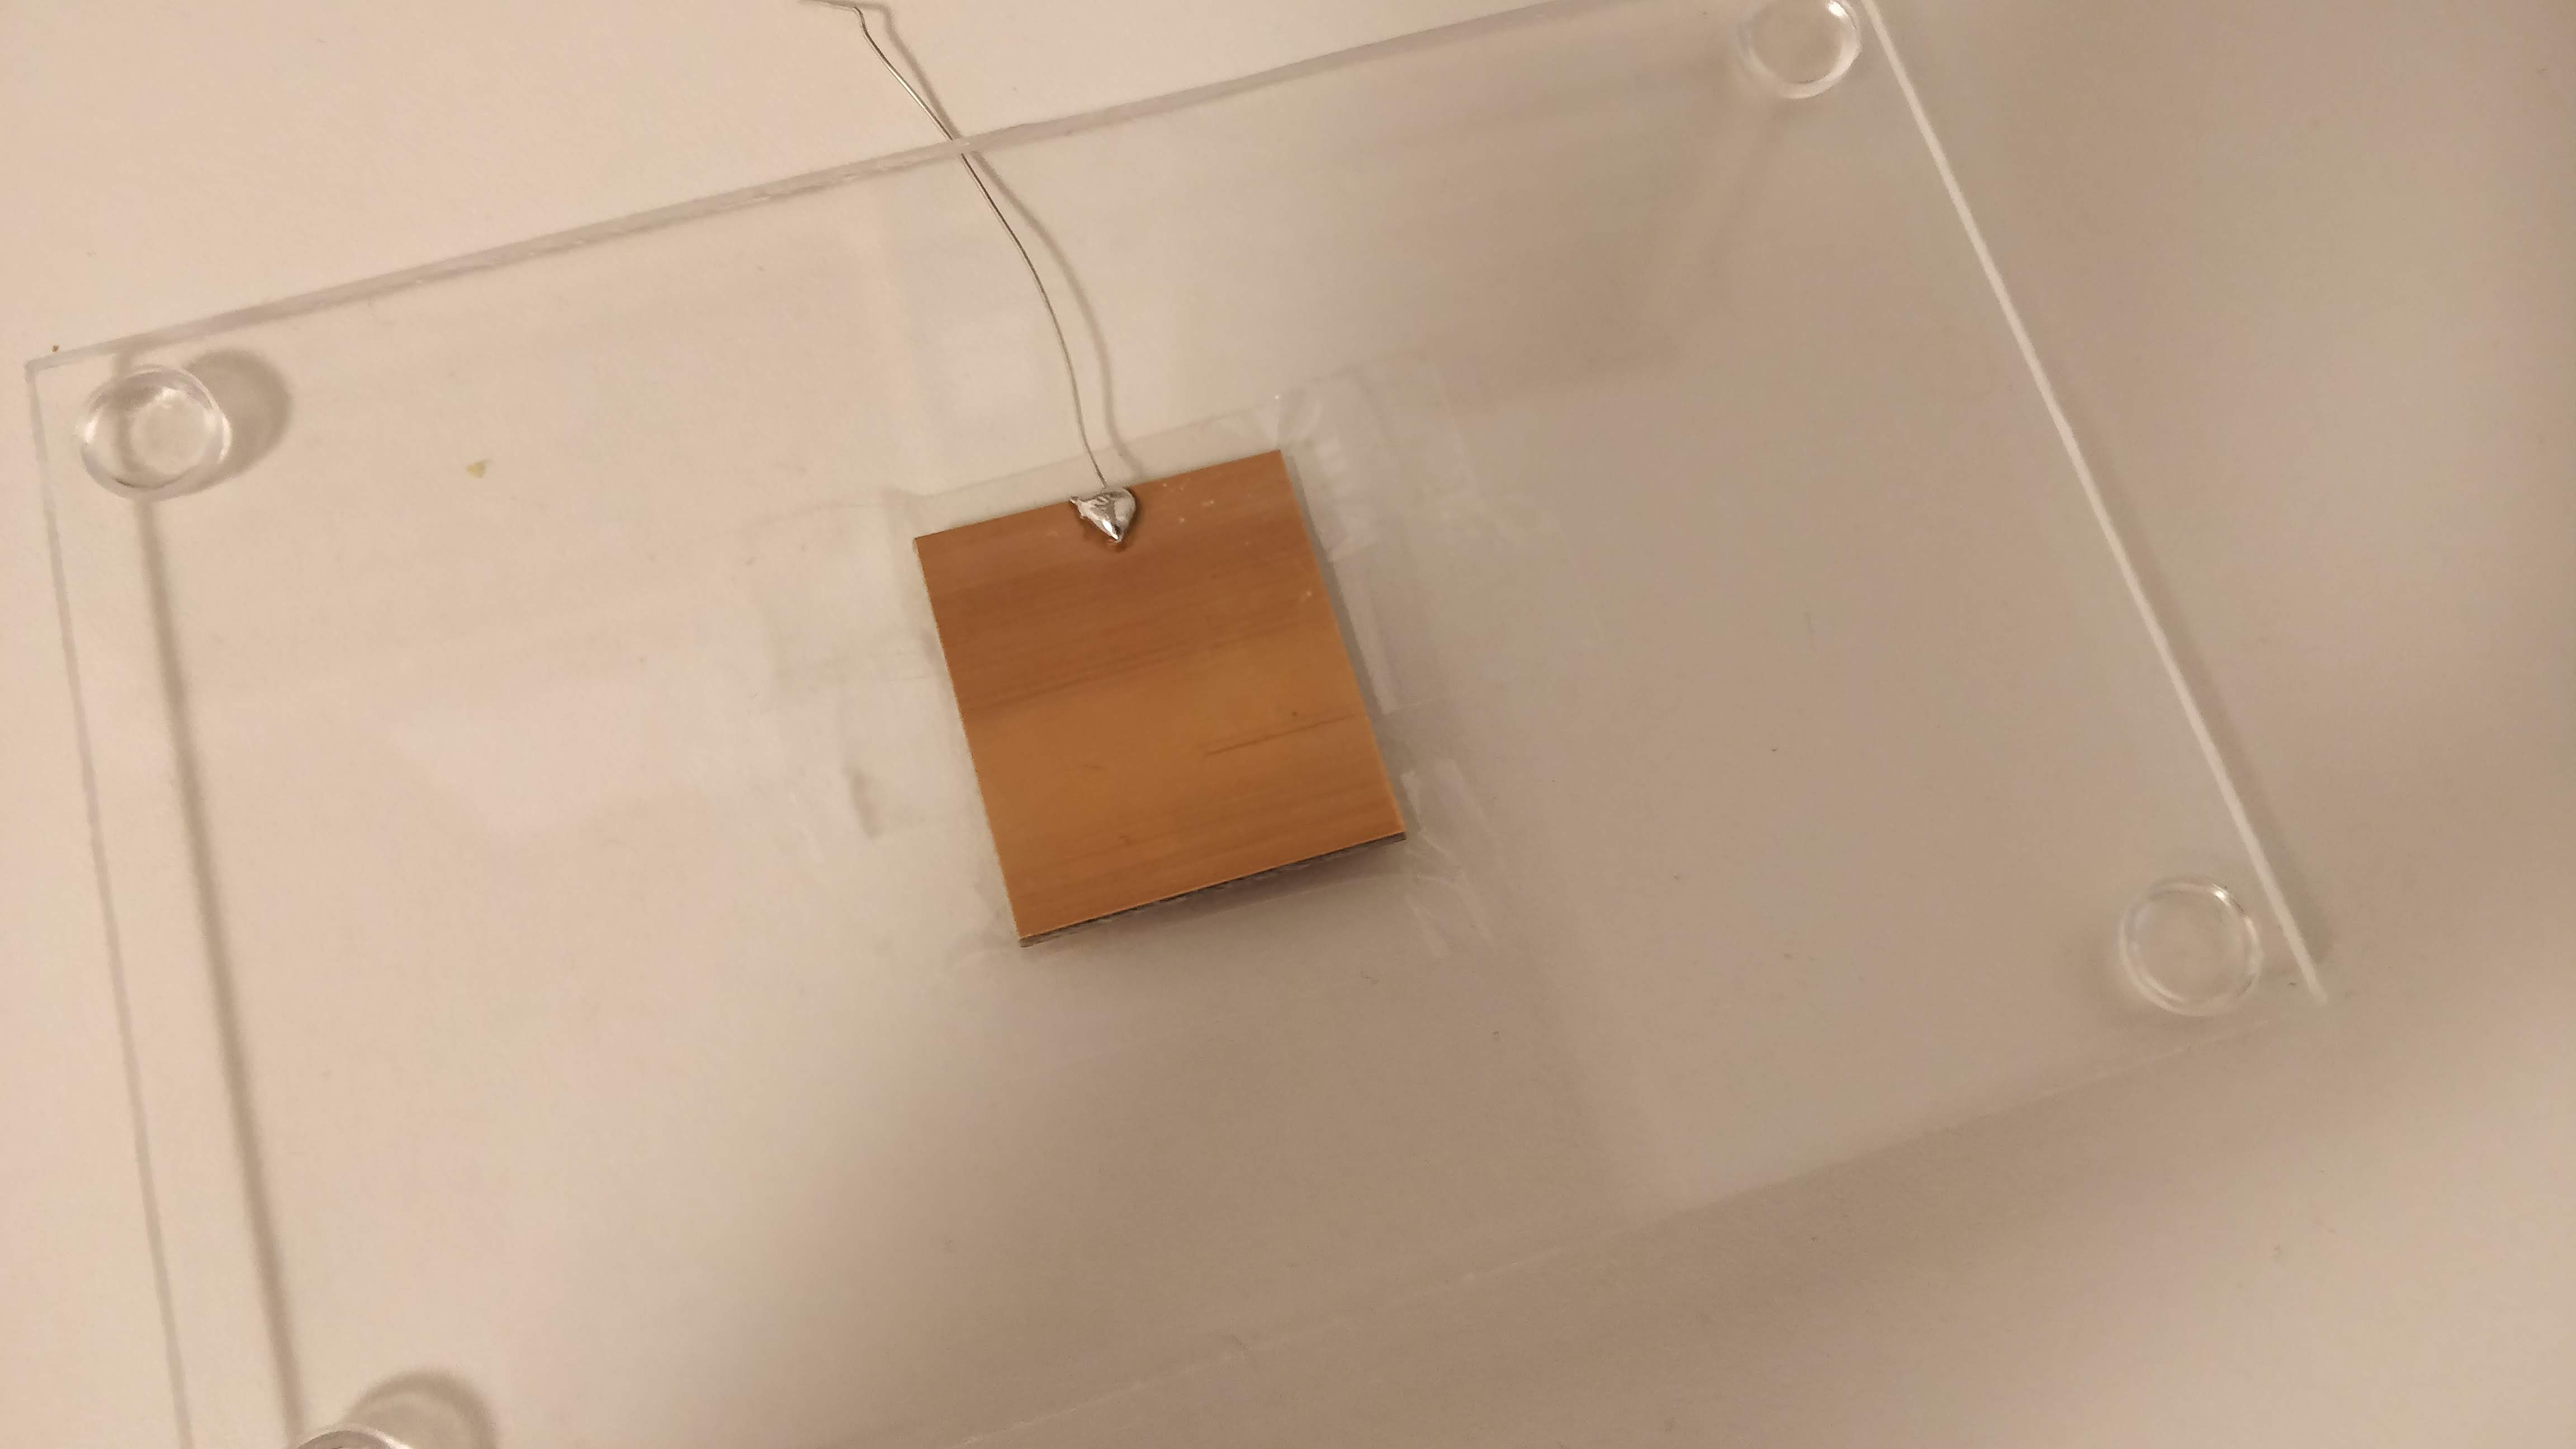
\includegraphics[width=0.8\textwidth]{HardwareDesign/CupSensor/graphics/CapTest/tape_plate.jpg}
    \caption{Akrylplade hvor der er tapet en kopperplade på ca 30mmx33mm på undersiden.}
    \label{fig:cap_tape_testopstilling}
\end{figure}

\begin{figure}[H]
    \centering
    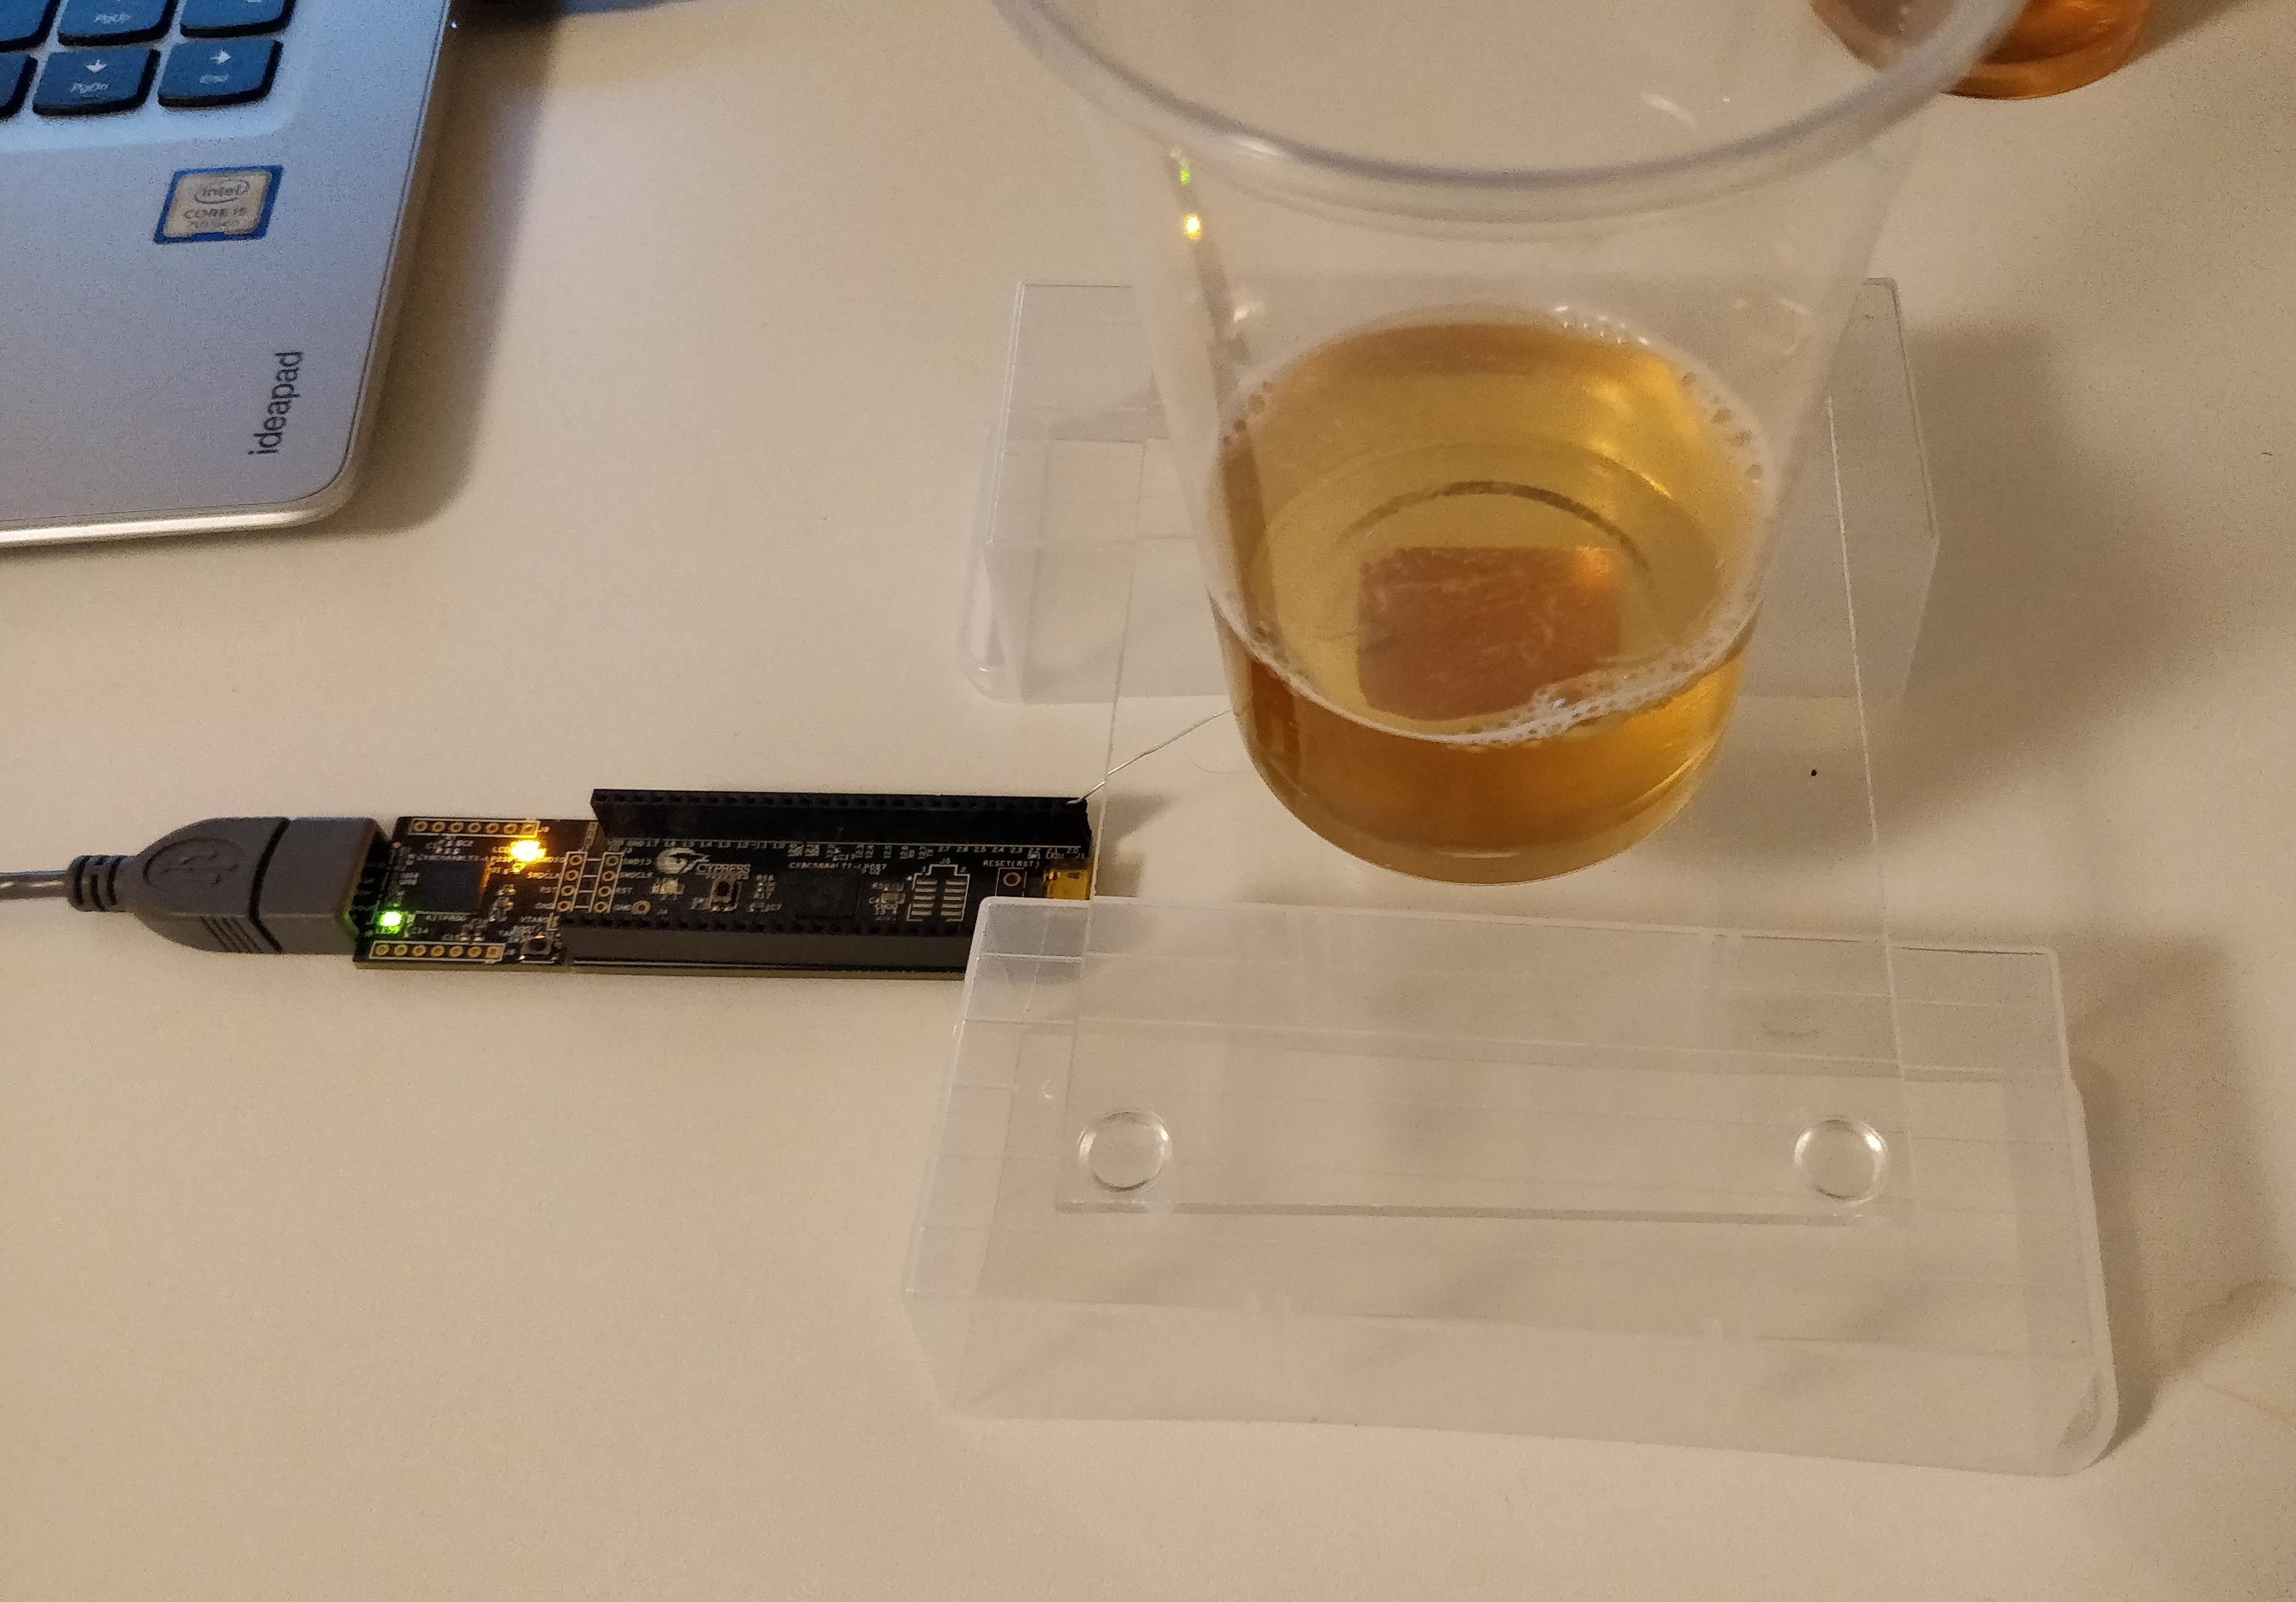
\includegraphics[width=0.8\textwidth]{HardwareDesign/CupSensor/graphics/CapTest/cap_testopstiling.jpg}
    \caption{Kopperplade fra \ref{fig:cap_tape_testopstilling} er nu forbundet til PSoC'en og det er vist hvor koppen vil blive placeret.}
    \label{fig:cap_testopstilling}
\end{figure}
\newpage
\textbf{Målinger ved 110ml øl}
\begin{figure}[H]
    \centering
    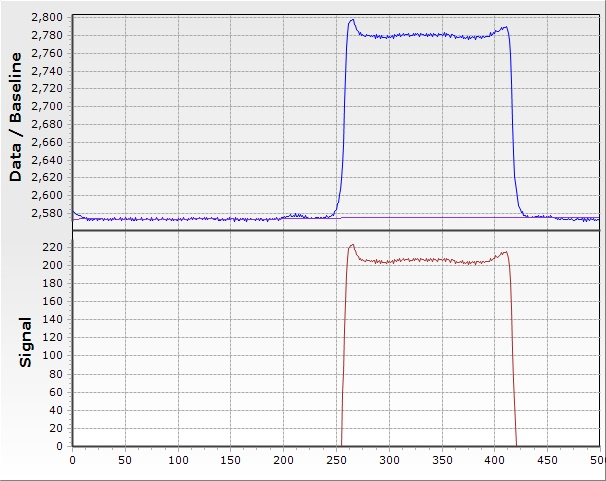
\includegraphics[width=\textwidth]{HardwareDesign/CupSensor/graphics/CapTest/placingAndRemovingCup1(beer).jpg}
    \caption{Test resultat ved placering (ca ved x=250) og fjernelse af kop (ca ved x=425). Øverste halvdel: rådata. Nederste halvdel: signal data, beregnet ud fra baseline}
    \label{fig:cap_test_place_and_remove_110}
\end{figure}

\begin{figure}[H]
    \centering
    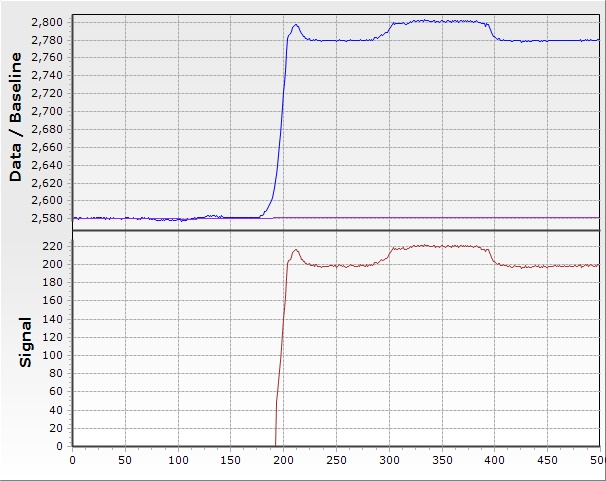
\includegraphics[width=\textwidth]{HardwareDesign/CupSensor/graphics/CapTest/placingCupAndPutingHandOnTop1(beer).jpg}
    \caption{Test resultat ved placering af kop (ca ved x=200) og placering af en flad hånd på toppen af koppen (ca ved x=300) og fjernelse af hånd (ca ved x=400). Øverste halvdel: rådata. Nederste halvdel: signal data, beregnet ud fra baseline}
    \label{fig:cap_test_place_and_hand_110}
\end{figure}

\begin{figure}[H]
    \centering
    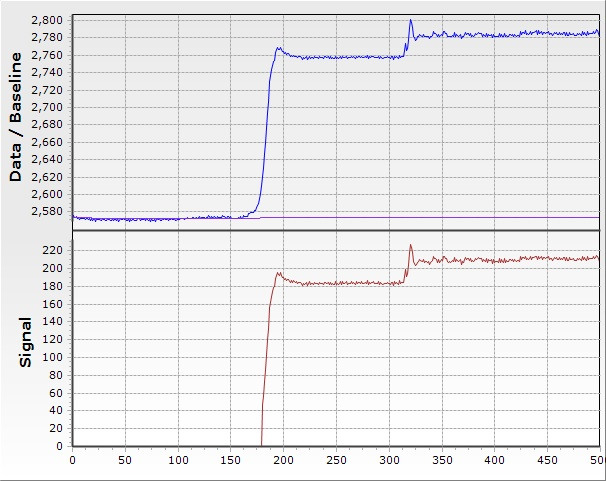
\includegraphics[width=\textwidth]{HardwareDesign/CupSensor/graphics/CapTest/placingCupAndDroppingBall1(beer).jpg}
    \caption{Test resultat ved placering af kop (ca ved x=185) og bold som rammer i koppen (ca ved x=320). Øverste halvdel: rådata. Nederste halvdel: signal data, beregnet ud fra baseline}
    \label{fig:cap_test_place_and_drop_110}
\end{figure}

\textbf{Målinger ved 220ml øl}
\begin{figure}[H]
    \centering
    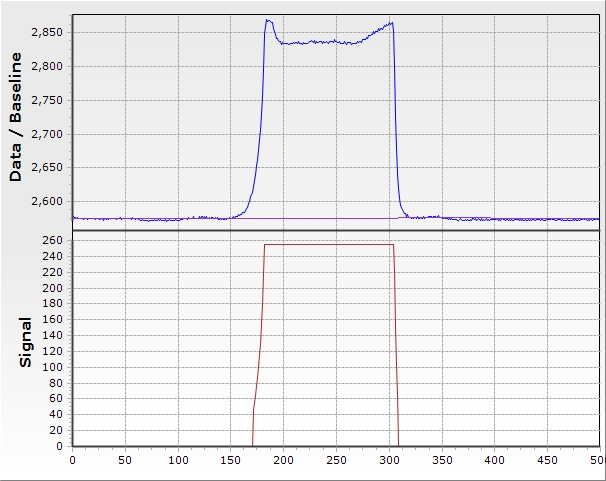
\includegraphics[width=\textwidth]{HardwareDesign/CupSensor/graphics/CapTest/placingAndRemovingCup2(beer-220ml).jpg}
    \caption{Test resultat ved placering (ca ved x=175) og fjernelse af kop (ca ved x=300). Øverste halvdel: rådata. Nederste halvdel: signal data, beregnet ud fra baseline}
    \label{fig:cap_test_place_and_remove_220}
\end{figure}


\begin{figure}[H]
    \centering
    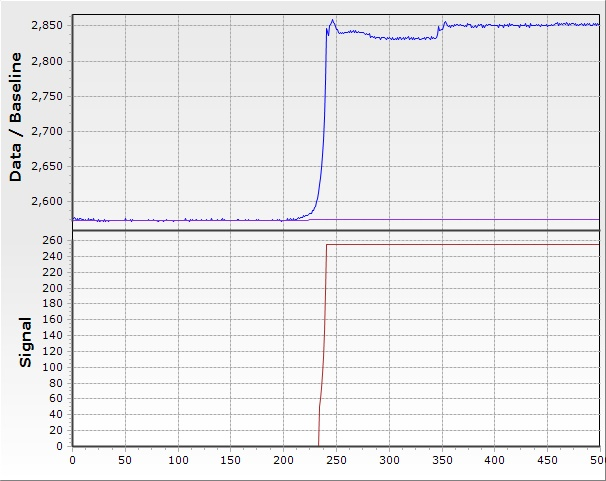
\includegraphics[width=\textwidth]{HardwareDesign/CupSensor/graphics/CapTest/placingCupAndDroppingBall1(beer-220ml).jpg}
    \caption{Test resultat ved placering af kop (ca ved x=240) og bold som rammer i koppen (ca ved x=350). Øverste halvdel: rådata. Nederste halvdel: signal data, beregnet ud fra baseline}
    \label{fig:cap_test_place_and_drop_220}
\end{figure}

\textbf{Diskussion af resultater}\\
Der ses på figur \ref{fig:cap_test_place_and_remove_110} at det er tydeligt om der er en kop eller ej. Det ses også at der kommer en spids når koppen placeres og når den fjernes, dette observeres også ved gentagne målinger. Dette kan muligvis skyldes at en hånd kommer i nærheden af sensoren. Det blev ikke målt, men det ses også at der er et relativ lavt signal-støjforhold (SNR), i forhold til den optiske sensor som undersøges i næste afsnit.

På figur \ref{fig:cap_test_place_and_hand_110} ses det der kommer en ændring i signalet når der placeres en hånd på toppen af koppen. Der aflæses fra grafen (den nederste halvdel) at signalet ca. stiger med $\frac{20}{200} = 10\%$. Der ses desuden af signalet stiger til ca. det samme niveau som spidsen ved placering af koppen, dette kan muligvis være med til at forklare at spidsen skyldes at der benyttes en hånd til at placere koppen.

På figur \ref{fig:cap_test_place_and_drop_110} ses det at der kommer en ændring i den stationære værdi når en bold rammer i koppen. Der aflæses fra grafen (den nederste halvdel af figur \ref{fig:cap_test_place_and_drop_110}) at den stationære værdi ca. stiger med $\frac{30}{180} = 17\%$. Der ses også at der kommer en spids idet bolden rammer i koppen, denne spids er ca $\frac{40}{180} = 22\%$ mere end signalet hvor der kun er en kop. Forøgelsen af signalet kan skyldes at bolden vil forøge den samlede overflade areal af øllen og dermed vil øge den frie kapacitet. Dette kan indikere at det måske er muligt at detektere en bold, da der er en ændring i signalet.

På figur \ref{fig:cap_test_place_and_remove_220} og figur \ref{fig:cap_test_place_and_drop_220} ses nogenlunde den samme for rådataen (øverste halvdel), udover at den procentvise ændring når bolden rammer i er mindre. Men det observeres også at signalet beregnet ud fra baseline (nederste halvdel af figurerne) er for stort, da det kun er 8 bit. Hvis der skal arbejdes videre med denne metode er det derfor vigtigt at få kalibreret og indstillet CapSense rigtigt.

\subsubsection{Optisk sensor}
Til at lave en optisk sensor benyttes en IR LED samt en eller flere fotodioder som er sensitive over for IR lys. Der benyttes kredsløbet som ses på \ref{fig:optic_test_diagram}. Operationsforstærkeren fungerer som en strømforstærker, som forstærker strømmen fra fotodioden og laver den om til en spænding. Spændingen ved AmpOut måles vha. Digilent Analog Discovery 2\autocite{AnalogDiscovery2}. Der er i denne undersøgelse en IR LED (SFH485\autocite{SFH485}) i centrum af koppen og og to fotodioder (SFH203FA\autocite{SFH203FA}) i siderne som det ses på figur \ref{fig:optic_opstilling}. 
\begin{figure}[H]
    \centering
    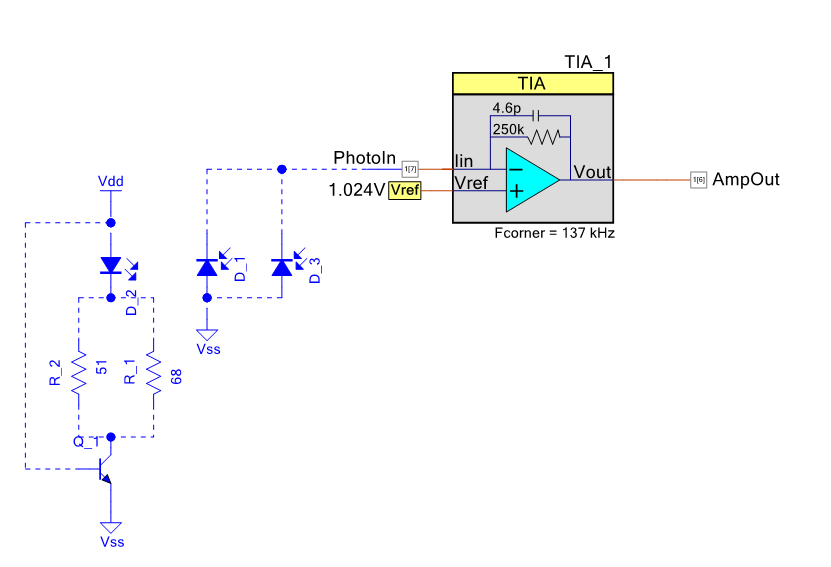
\includegraphics[width=\textwidth]{HardwareDesign/CupSensor/graphics/OpticTest/diagram.PNG}
    \caption{Test kredsløb for optisk sensor}
    \label{fig:optic_test_diagram}
\end{figure}

\begin{figure}[H]
    \centering
    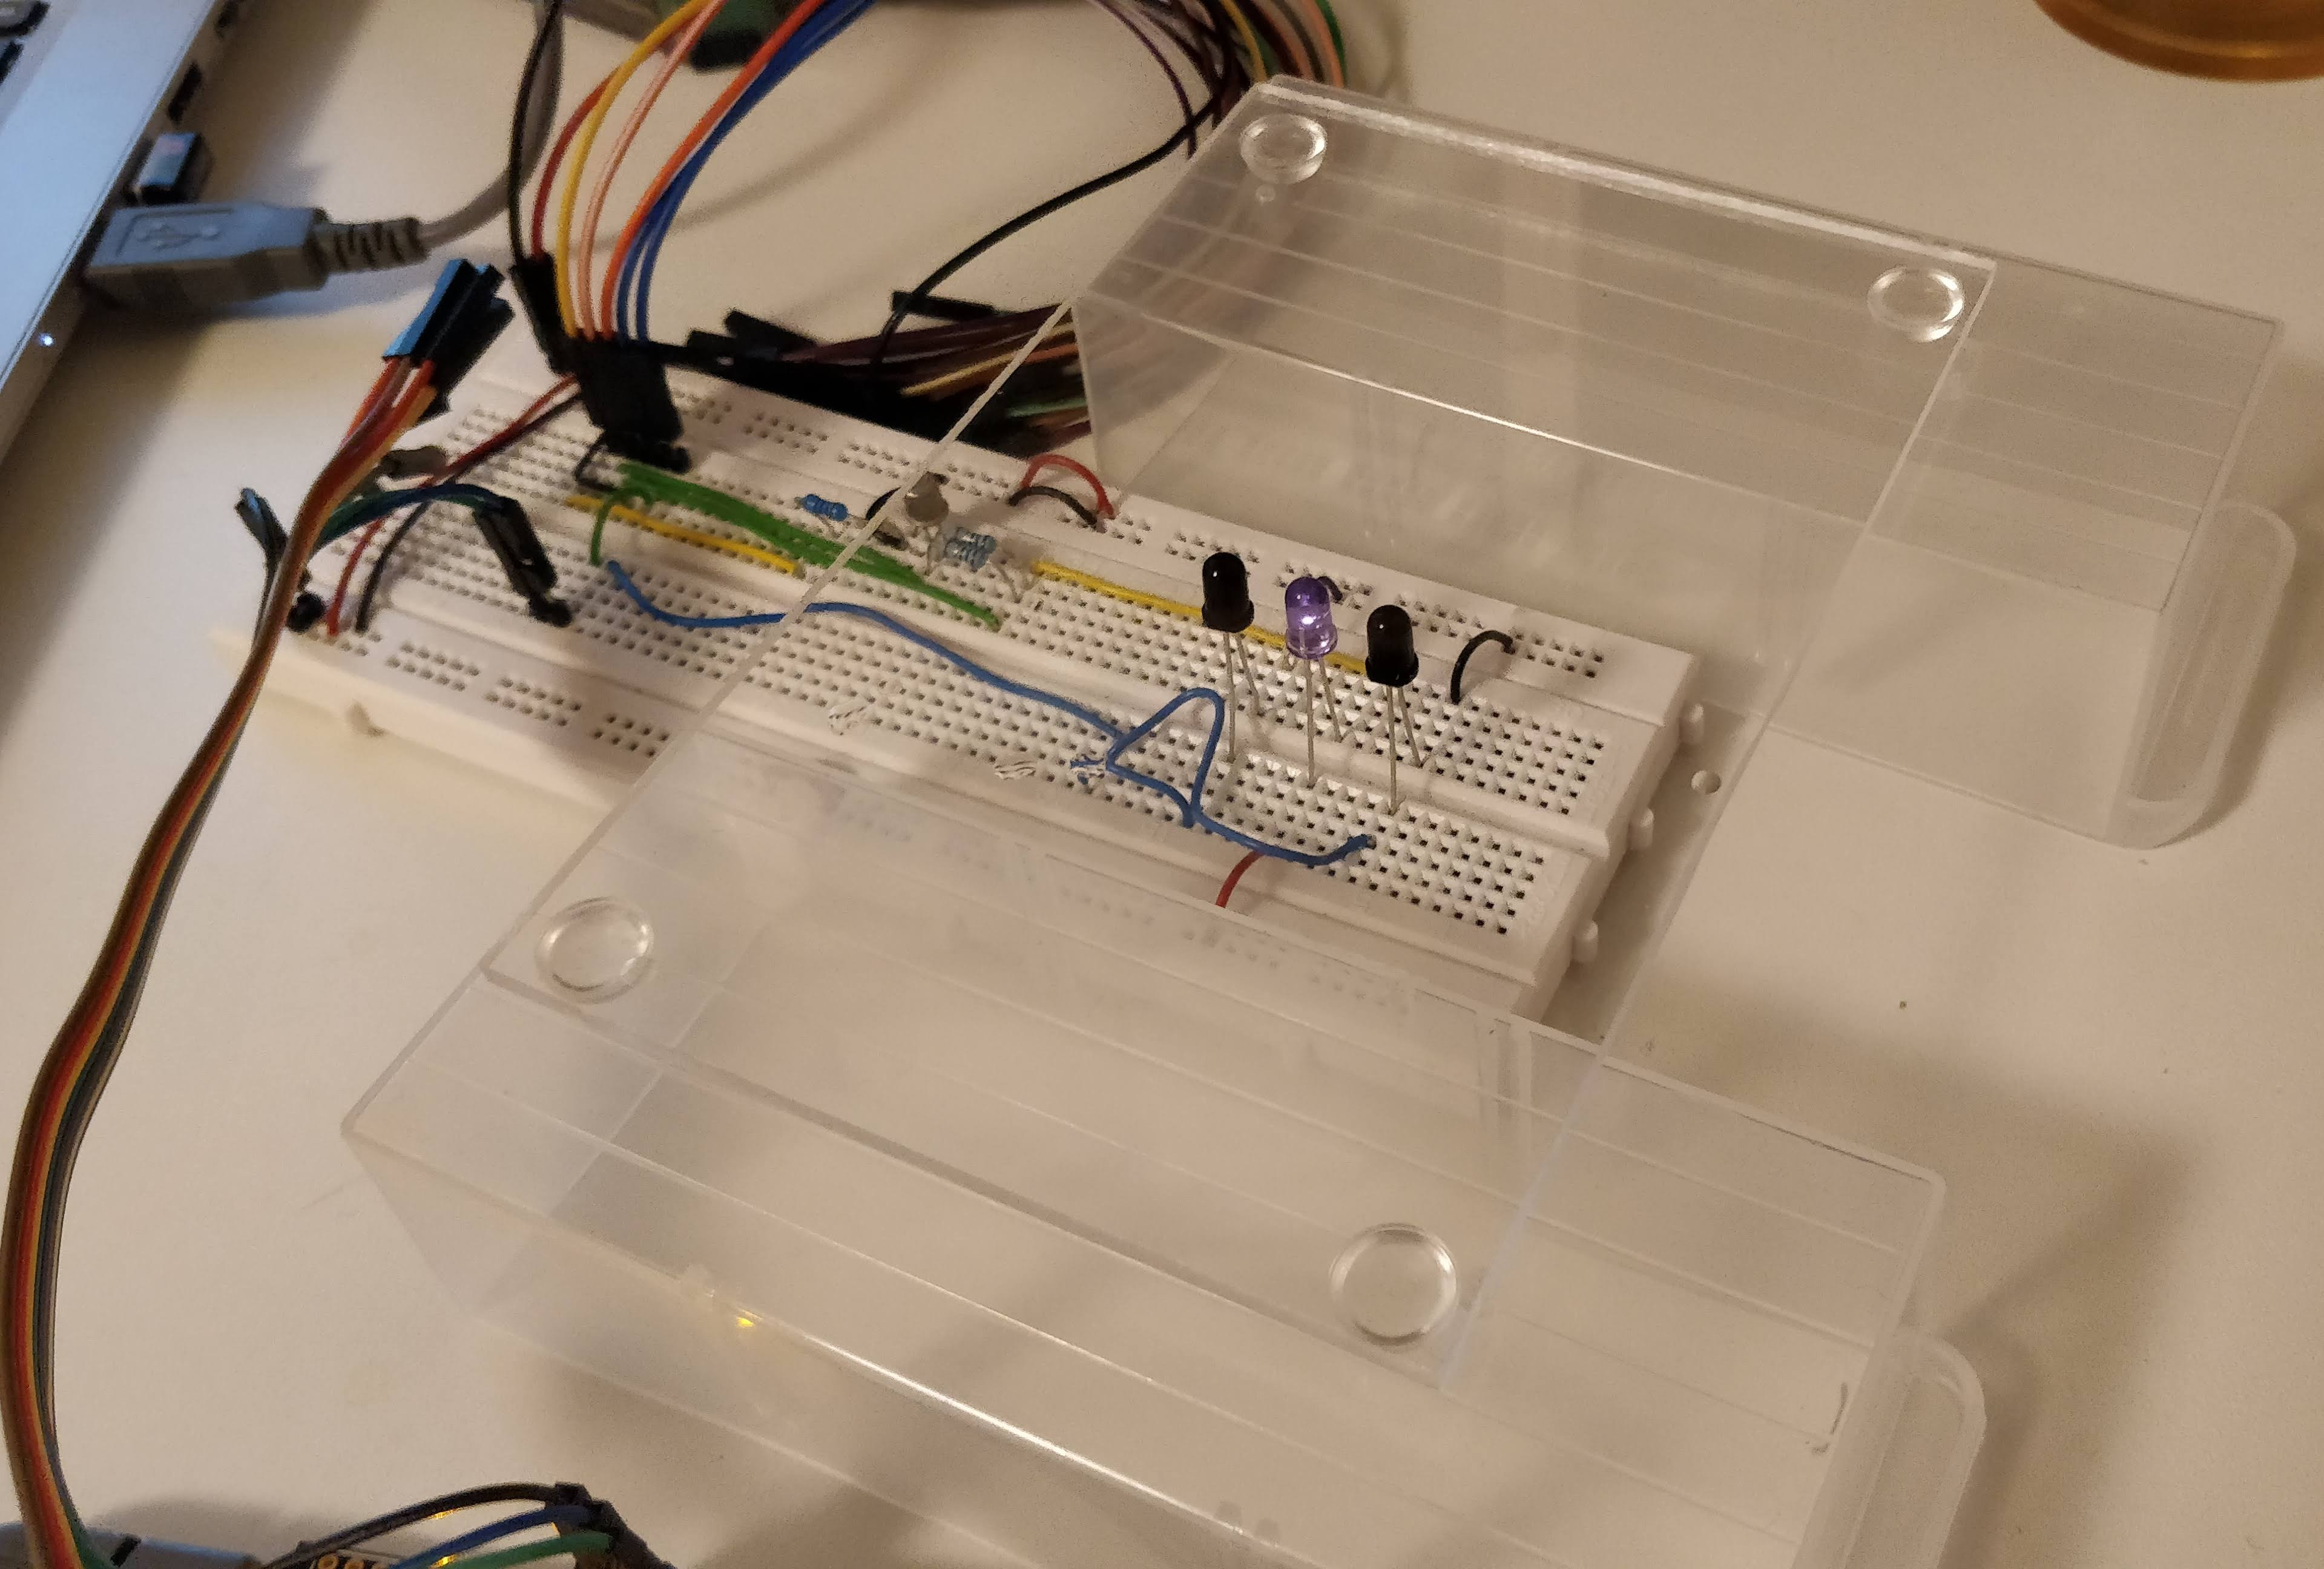
\includegraphics[width=\textwidth]{HardwareDesign/CupSensor/graphics/OpticTest/Optic_testopstillign.jpg}
    \caption{Test opstilling for optisk sensor. Den lilla diode er den infrarøde LED og de to sorte er fotodioderne. Der er ligesom for den kapacitive sensor en akrylplade som koppen placeres på}
    \label{fig:optic_opstilling}
\end{figure}

Til at lave målinger der er sammenlignelige med de målinger der laves til den kapacitive sensor, skal den bedste afstand mellem IR LED og fotodioder bestemmes. Dette gøres ved at måle signalet når der ikke er en kop, når der er en kop med øl, når der er en bold som flyder i øllen i centrum af koppen og når der er en bold som flyder i øllen i kanten af koppen (over en af fotodioderne). Disse målinger udføres ved afstande mellem IR LED og hver af fotodioderne i intervallet 7mm til 28mm. Resultatet kan ses på \ref{fig:optic_test_afstand_raw}, hvor spændingen i forhold til referencen på 1.024V er plottet.
Målingen uden en kop, kan sammenlignes med det Cypress kalder baseline i CapSense. Denne måling trækkes fra de andre målinger. Herefter fås det der ses på figur \ref{fig:optic_test_afstand}. Derudover beregnes også den procentvise ændring ved at der er en bold i koppen. Dette kan ses på figur \ref{fig:optic_test_afstand_procent}

\begin{figure}[H]
    \centering
    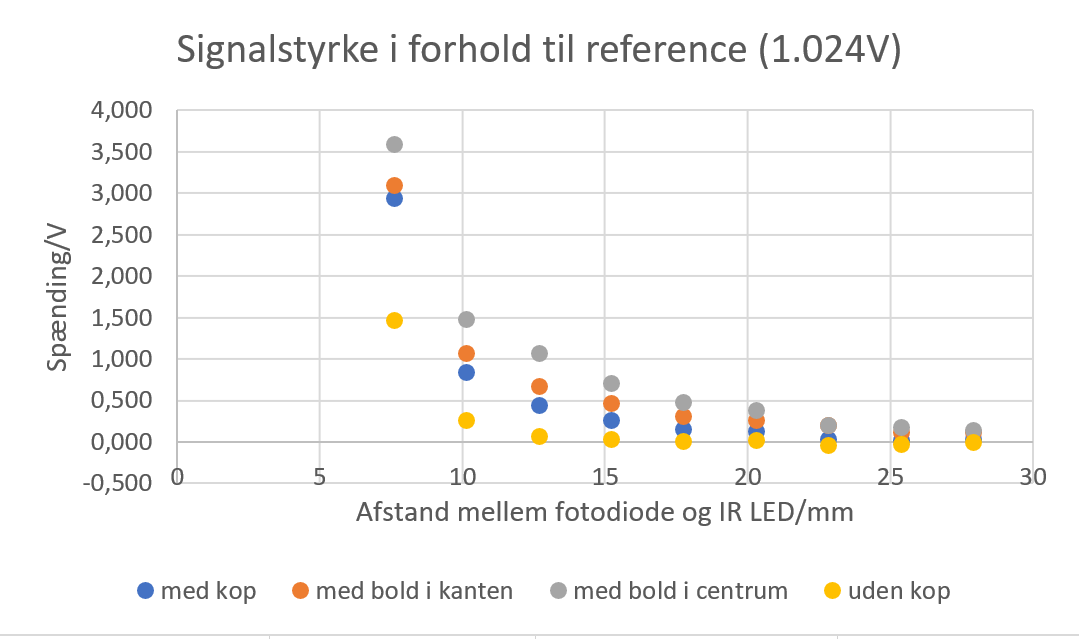
\includegraphics[width=\textwidth]{HardwareDesign/CupSensor/graphics/OpticTest/beer_afstand_raw.PNG}
    \caption{Testresultater, der viser signalstyrken i forhold til referencen på 1.024V som funktionen af afstanden mellem LED og fotodiode}
    \label{fig:optic_test_afstand_raw}
\end{figure}

\begin{figure}[H]
    \centering
    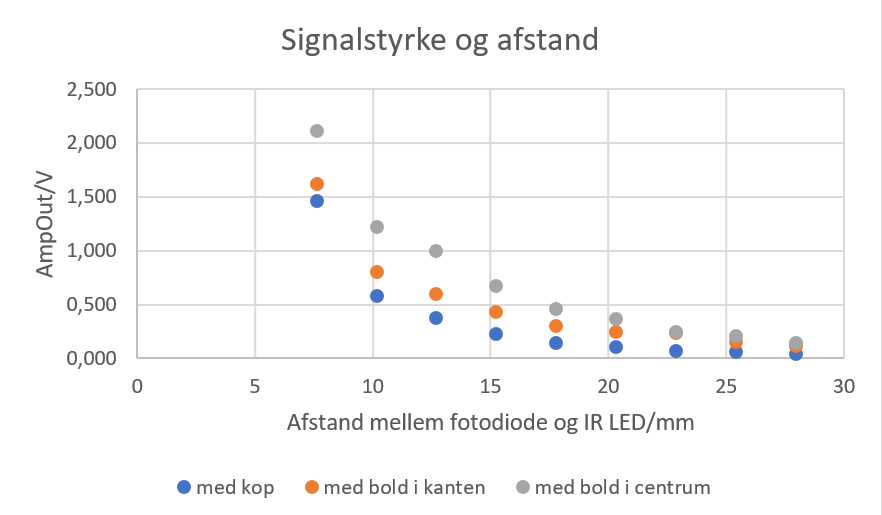
\includegraphics[width=\textwidth]{HardwareDesign/CupSensor/graphics/OpticTest/beer_afstand.PNG}
    \caption{Testresultater, der viser signalstyrken som funktionen af afstanden mellem LED og fotodiode}
    \label{fig:optic_test_afstand}
\end{figure}

\begin{figure}[H]
    \centering
    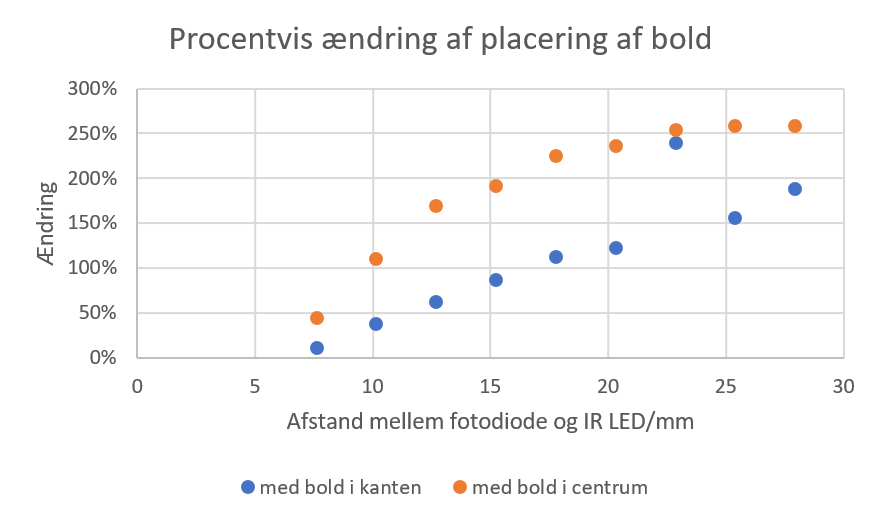
\includegraphics[width=\textwidth]{HardwareDesign/CupSensor/graphics/OpticTest/beer_afstand_procent.PNG}
    \caption{Testresultater, der viser den procentvise ændring ved at tilføje en bold til koppen som funktionen af afstanden mellem LED og fotodiode}
    \label{fig:optic_test_afstand_procent}
\end{figure}

Der ses på figur \ref{fig:optic_test_afstand} at signalet bliver større jo tættere dioderne er på hinanden. Desuden ses det på \ref{fig:optic_test_afstand_raw} at 'baseline' signalet (signalet uden en kop) også stiger jo tættere dioderne er på hinanden. Derudover ses det på figur \ref{fig:optic_test_afstand_procent} at der sker en større procentvis ændring i signalet, når der er en bold i koppen, jo længere dioderne er fra hinanden. Sensorens hovedformål er at detektere placering af en kop, der skal derfor være et relativt stort og pålideligt signal når der er en kop. Derfor vælges det at arbejde videre med afstanden på ca 10mm, her er et relativt stort signal, sammenlignet med en peak-peak støjværdi på ca 40mV. Der er stadig en relativ stor procentvis ændring på 38\% til 110\%. Sammenlignet med 17\% for den kapacitive sensor.

Der testes nu den transiente respons ved placering af kop og ved tab af bold i kop. På figur \ref{fig:optic_place_and_drop_110ml} vises resultatet af at placere en kop på sensoren efterfulgt af at tabe en bold i koppen.

\begin{figure}[H]
    \centering
    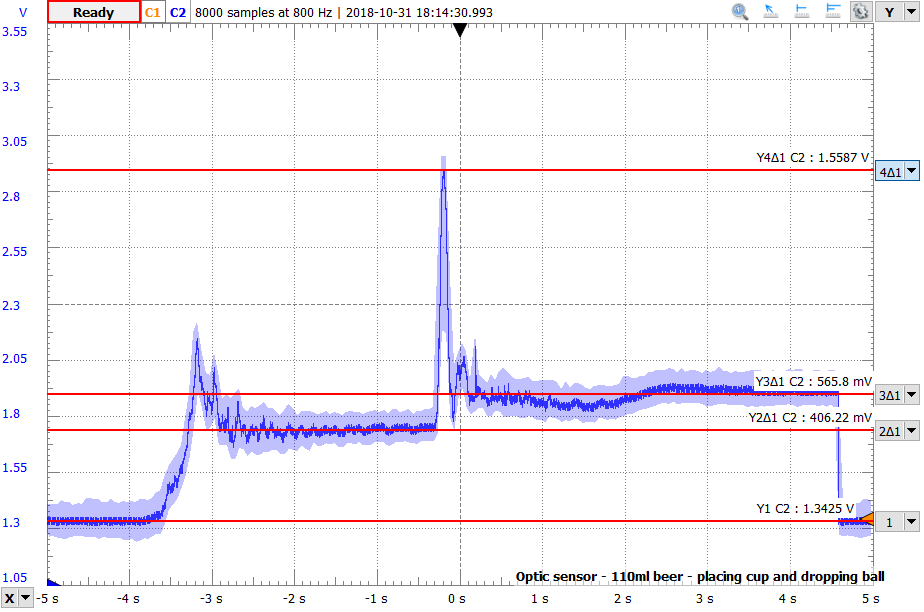
\includegraphics[width=\textwidth]{HardwareDesign/CupSensor/graphics/OpticTest/placingCupAndDroppingBall(110ml-beer).png}
    \caption{Transient repsons for placering af kop (ca ved t=-3,5s)  og tab af bold (ca ved t=-0,3s)}
    \label{fig:optic_place_and_drop_110ml}
\end{figure}


\textbf{Diskussion af resultater}\\
Der ses på \ref{fig:optic_place_and_drop_110ml} at der kommer en spids, når der placeres en kop. Denne spids kommer også over der stationære niveau for når der er en bold i koppen. Derudover kommer der en meget stor spids når bolden rammer i koppen. Dette kan muligvis forklares ved at bolden kommer meget tæt på LED og fotodiode. Denne spids er meget stor, det er en procentvis ændring fra når der er en kop på ca $\frac{1.1\si{V}}{0.4\si{V}} = 275\%$, hvilket er meget større end den kapacitive sensor på ca. 22\%. Denne spids kan derfor bruges til at detektere at en bold rammer i. 

\subsubsection{Signal-støjforhold}
Som en del af valg af den bedste teknologi (næste afsnit) diskuteres der bl.a. signal-støjforhold for den kapacitive sensor og den optiske sensor. Disse diskussioner bygger ikke på det bedste grundlag, da målingerne blev udført før et ordentligt kendskab til signal-støjforhold, og der blev derfor ikke målt RMS værdien af støjen. Der laves dog stadig overvejelser omkring signal-støjforholdet, ud fra det man kan se på graferne. Hvis man sammenligner de to grafer som ses på \ref{fig:optic_place_and_drop_110ml} og øverst på figur \ref{fig:cap_test_place_and_drop_110} ses det at der er mere støj for den optiske sensor i forhold til hvor stor signal ændring der er (ændring mellem der hvor der ikke er en kop, og der hvor der er en kop). For optiske sensor er der en tyk 'streg' hvilket betyder at der meget støj, da signalet svinger meget op og ned, hvorimod der er en meget tynd 'streg' for den kapacitive sensor. Disse observationer kan derfor indikere at den kapactive sensor har et større signal-støjforhold. Dog er der desvære ikke målinger der efterviser dette.

\subsubsection{Valg af teknologi}
Begge teknologier virker til at være i stand til at detektere at at kop placeres på og muligvis også at en bold rammer i.
Der vælges nu en af de to teknologier. Den kapcitive sensor har et højere signal-støjforhold (SNR) end den optiske sensor. Hvis der udelukkende vælges på bagrund af SNR, vil det være bedst at vælge den kapacitive sensor. Men da det også er et 'should' krav at være i stand til at detektere at en bold rammer i koppen, medtages muligheden for dette også i valget af teknologi. Undersøgelserne viste at der med den kapcitive sensor ikke kommer den store ændring i signalet når en bold rammer i. Med den optiske sensor er der en større ændring, og en endnu større kortvarig ændring, det vil derfor være nemmere at detektere at en bold rammer i vha. den optiske sensor. Desuden er det ud fra undersøgelsen af den optiske sensor muligt at justere hvor stor ændring der skal være (på bekostning af SNR). Dette vil muligvis også være muligt med den kapacitive sensor, men det er svært at analysere sig frem til den bedste løsning, og omkostningsfuldt at teste mange forskellige løsninger (både tid og ressourcer). 

Sensoren skal kun detektere 3 forskellige tilstande: der er ikke en kop, der er en kop og der er en kop med en bold i. Dette kræver ikke nødvendigvis så stor en SNR. Hvis der derimod skulle måles hvor meget øl der er i en kop, vil det være vigtigt med en høj SNR. Med den optiske sensor er der større ændring i signalet når en bold rammer i.

En meget stor fordel for den kapacitive sensor er at den er meget billig, der skal kun benyttes en PSoC (som allerede skal bruges til andre dele af systemet) og en metal plade, dette kan nemt være som en del af en større printplade. Hvis der i en senere model ikke ønskes at bruge PSoC og dermed CapSense, kan det måske løses med en billigere løsning. Det kan måske være muligt at måle kondensatoren vha. et simpelt RC led, hvor stigetiden måles. Det kan derfor være meget billigt med en kapacitiv sensor. Til en optisk sensor skal der derimod benyttes en del flere komponenter som dermed gør systemet dyrere.
Det er svært at vælge en teknologi på grundlag af prisen, da der ikke er sat nogen specifikke krav til prisen af produktet. Derfor vælges den optiske sensor, da det gør det meget realistisk at være i stand til at detektere både en kop og at en bold rammer i.

\subsubsection{Diskussion} \label{sec:CupSensorTekUnderDiskussion}
Undervejs i teknologiundersøgelsen blev der observeret forskellige ting som er interesant til den videre udvikling. 
I testen hvor forholdet mellem signalstyrke og afstanden mellem LED og fotodiode blev undersøgt, blev det observeret at signalet varierer afhængig af hvor i kanten bolden er. Altså hvis bolden er lige over en fotodiode er signalet højt, men hvis den drejes 90 grader rundt om centrum af koppen, så den er midt i mellem de to fotodioder (men stadig i kanten af koppen), er signalet lavere. Ud fra dette kan det erfares at det vil være fordelagtigt at have flere fotodioder i en cirkel rundt om den infrarøde LED. Dette vil dog være spild at have alt for mange fotodioder, så det tænkes at 4 er tilstrækkelig.
Som en del af undersøgelsen af hvordan CapSense virker, blev deres signalbehandling beundret. Den måde CapSense detektere om der er en finger/kop/mm. vha. baselines virker som en smart signalbehandling. Det overvejes derfor at benyttes denne type signalbehandling til brug ved den optiske sensor.

\subsubsection{Konklusion} \label{sec:CupSensorTekUnderKonklusion}
I denne teknologiundersøgelse er der undersøgt specielt to forskellige teknologier, kapacitiv sensor og optisk sensor. Der blev valgt den optiske sensor, som er undersøgt nok til et 'proof of concept', der gør at der i den videre udvikling kan bevares en meget godt tiltro at teknologien vil virke. Men den skal stadig videreudvikles.

\iffalse
{
\subsection{Nærmere undersøgelse}
\subsubsection{Maksimal mulig strøm fra en fotodiode (uden AC coupling)} \label{sec:CupSensorCurrentTest}
{
Dette afsnit bygger på et design som det fra teknologiundersøgelsen. Dette er ikke det endelige design og dette afsnit er derfor ikke så brugbart længere. Det kan dermed springes over.

Til at bestemme om forskellige designs er mulige, er det nødvendigt at kende strømmen fra fotodioden i forskellige tilfælde.
Der benyttes fotodioden SFH 203 FA. I databladet for denne står der at photocurrent er $50 (\geq 30) \si{mA}$ men dette er for en bestem bølgelængde og lysintensitet. Det er ikke tydeligt om det er den maksimale strøm, derfor måles denne.
Det testes nu hvad den maksimal mulige strøm fotodioden kan levere når den direkte belyses af LED'en. Dette er ikke nødvendigvis det maksimale den kan levere, men det antages at fotodioden aldrig vil blive belyst med mere end dette.
LED'en tændes og strømmen måles ved hjælp af kredsløbet som ses på figur \ref{fig:PhotodiodeTestDiagram}. Strømmen måles ved at måle spændingen over formodstanden. Formodstanden er en parallel kobling af en 68Ohm modstand og en 51Ohm modstand som svare til 29Ohm. Spændingen over modstandene måles til $3.06\si{V}$ og dermed er den samlede strøm gennem dem og dermed LED'en ca $106\si{mA}$. Denne strøm måles da det er ca denne strøm der regnes med at blive brugt. Strømmen fra fotodioden måles vha. TIA'en som ses på figur \ref{fig:PhotodiodeTestDiagram}. Her måles spændingen $4.65V$. Dette er det maksimale output af TIA'en og forstærkningen kan ikke sænkes. Ud fra dette resultat kan det konkluderes at strømmen fra photdioden mindst er $230\si{\mu A}$

\begin{figure}[H]
    \centering
    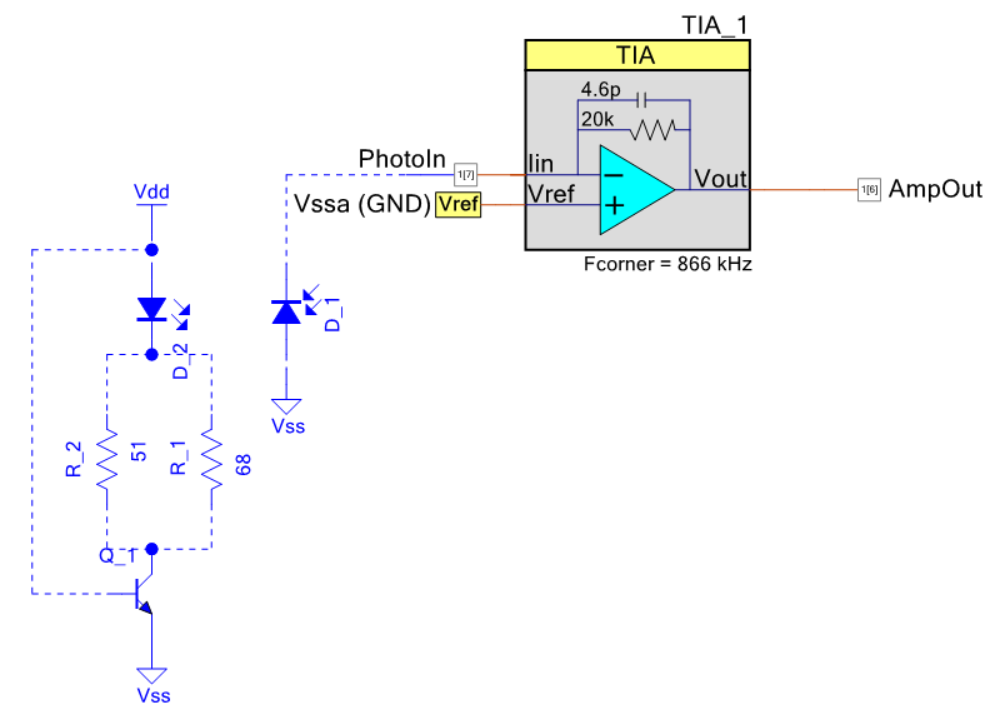
\includegraphics[width=\textwidth]{HardwareDesign/CupSensor/graphics/DiodeCurrentTestDiagram.PNG}
    \caption{Diagram for test kredsløb}
    \label{fig:PhotodiodeTestDiagram}
\end{figure}

Opstillingen ændres nu til det som ses på figur \ref{fig:CurrentTestUpDown}. TIA'ens feedback modstand ændres til $40\si{k\Omega}$ Der benyttes et spejl som bevæges op og ned over photodiode/LED og den maksimale værdi fra TIA'en bestemmes til $3.89\si{V}$. Den maksimale strøm med denne opstilling er derfor $97\si{\mu A}$.

Der benyttes nu samme opstilling men der benyttes en plastikkop med en bordtennisbold (her måles en større strøm end en kop med væske) i stedet for et spejl. TIA'ens feedback modstand ændres til $120\si{k\Omega}$. Koppen bevæges op og ned over photodiode/LED og den maksimale værdi fra TIA'en bestemmes til $2.98\si{V}$. Den maksimale strøm med denne opstilling er derfor $25\si{\mu A}$.

Der benyttes nu opstillingen som kan ses på figur \ref{fig:CurrentTestBeer}. Der er 110ml øl i koppen. TIA'ens feedback modstand ændres til $250\si{k\Omega}$. En bordtennis bold kastes ned i koppen den maksimale værdi fra TIA'en bestemmes til $1.86\si{V}$. Den maksimale strøm med denne opstilling er derfor $7.4\si{\mu A}$.

Der benyttes nu samme opstilling men akrylpladen flyttes helt ned til LED/fotodiode (før var den ca $4\si{mm}$ fra LED/fotodiode) \ref{fig:CurrentTestBeer}. TIA'ens feedback modstand er stadig $250\si{k\Omega}$. En bordtennis bold kastes ned i koppen den maksimale værdi fra TIA'en bestemmes til $1.82\si{V}$ (hvilket er stort set det samme som ved den tidligere test. Den maksimale strøm med denne opstilling er derfor $7.3\si{\mu A}$. \\
Det noteres desuden at spændingen fra TIA'en er $158\si{mV}$ (strømmen er dermed $0.6\si{\mu A}$ når der ikke er nogen kop, i modsætningen til når pladen er hævet ca $4\si{mm}$ hvor spændingen fra TIA'en er $675\si{mV}$ (strømmen er dermed $2.7\si{\mu A}$. Dette er ikke formålet med denne test, men det betyder at akrylpladen skal placeres så tæt på LED og fotodiode så muligt, da signalændringen bliver større når akrylpladen er tæt på LED og fotodiode. 

Der benyttes nu samme opstilling men der benyttes en hånd i stedet for en kop med øl. TIA'ens feedback modstand ændres til $120\si{k\Omega}$. Håndes bevæges op og ned over photodiode/LED og den maksimale værdi fra TIA'en bestemmes til $2.36\si{V}$. Den maksimale strøm med denne opstilling er derfor $20\si{\mu A}$.

Resultaterne vises på tabel \ref{tab:CupSensorCurrentTest}

\begin{table}[H]
\begin{tabular}{|L{0.25\textwidth}|L{0.25\textwidth}|L{0.25\textwidth}|L{0.25\textwidth}|}
\hline
\textbf{Måleopstilling} & \textbf{TIA feedback modstand} & \textbf{Maximal TIA udgangsspænding} & \textbf{Maksimal Strøm fra fotodiode} \\ \hline
\textbf{LED lyser ind i fotodiode} & $20\si{k\Omega}$ & $4.65\si{V}$ & $230\si{\mu A}$ \\ \hline
\textbf{Spejl} & $40\si{k\Omega}$ & $3.89\si{V}$ & $97\si{\mu A}$ \\ \hline
\textbf{Plastikkop med bold} & $120\si{k\Omega}$ & $2.98\si{V}$ & $25\si{\mu A}$ \\ \hline
\textbf{Plastikkop med bold, øl og akrylplade} & $250\si{k\Omega}$ & $1.86\si{V}$ & $7.4\si{\mu A}$ \\ \hline
\textbf{Plastikkop med bold, øl og akrylplade helt tæt på LED og fotodiode} & $250\si{k\Omega}$ & $1.82\si{V}$ & $7.3\si{\mu A}$ \\ \hline
\textbf{Hånd og akrylplade helt tæt på LED og fotodiode} & $120\si{k\Omega}$ & $2.36\si{V}$ & $20\si{\mu A}$ \\ \hline
\end{tabular}
\caption{Testresultater for forskellige opstillinger}
\label{tab:CupSensorCurrentTest}
\end{table}
}
}
\fi


\subsection{Detektering af lys}
Til at detektere lys bruges der som tidligere beskrevet en fotodiode som skal detektere lys fra en IR LED. 
Det er valgt at benytte fotodioden SFH203FA som er mest sensitiv overfor infrarødt lys (900 nm)\autocite[2]{SFH203FA} og passer meget godt til lyset som kommer fra LED'en SFH485 (880nm)\autocite[3]{SFH485}. Det er valgt at benytte infrarødt lys, da der i normale omgivelser vil være større forstyrelser i det synlige område, fx fra kunstig belysning. De valgte komponenter er valgt da de passer godt til hinanden samt at det er dem, som der er tilrådighed. 
Da der altid vil være forstyrelser fra andre kilder er det valgt at LED'en skal blinke med en given frekvens og der kun måles signaler fra fotodioden ved denne frekvens. Til dette vil der benyttes en mixer, som vil blive forklaret senere. 

Opstillingen der vil benyttes kan ses på figur \ref{fig:lightPath}. I teknologiundersøgelsen (afsnit \fullref{sec:CupSensorTekUnderDiskussion}) blev det bestemt at der skal benyttes 4 fotodioder. Disse er placeret rund om den infrarøde led. Afstanden mellem centrum på IR LED og en fotodiode skal være 4 modulafstande (10.16mm). På figur \ref{fig:lightPath} er der påtegnet hvordan det forventes lyset bevæger sig. Lyset fra IR LED udsendes hovedsagligt op ad. Ved $20^\circ$ i forhold til lodret, udsendes der kun 50\% af lysintensiteten i forhold til den maksimale (som er op ad)\autocite[3, 8]{SFH485}. For fotodioden gælder der det samme. ved $20^\circ$ detekteres der 50\% så meget som hvis lyset kom oppe fra. af lyset\autocite[2,6]{SFH203FA}. Det kan frygtes at lyset bevæger sig direkte fra IR LED til fotodiode. Men ved en vinkel på $90^\circ$ detekteres der kun omkring 5\% så meget som ved lodret\autocite[6]{SFH203FA} og der udsendes kun omkring 2\%\autocite[8]{SFH485}. Kombineres disse to har det ikke den store indflydelse. Det samme gælder det lys som reflekteres på plastikpladen. Det der er i en lille nok vinkel til at have en markant lysstyrke vil, som det ses på figur \ref{fig:lightPath}, ikke ramme fotodioderne. Derimod vil lys som reflekteres på øloverflade, eller bold overflade, være i stand til at ramme fotodioden, som det ses på \ref{fig:lightPath}. Dog vil ikke alt lyset blive reflekteret. Disse beskrivelser er dog kun den måde det antages at lyset bevæger sig på.

\begin{figure}[H]
    \centering
    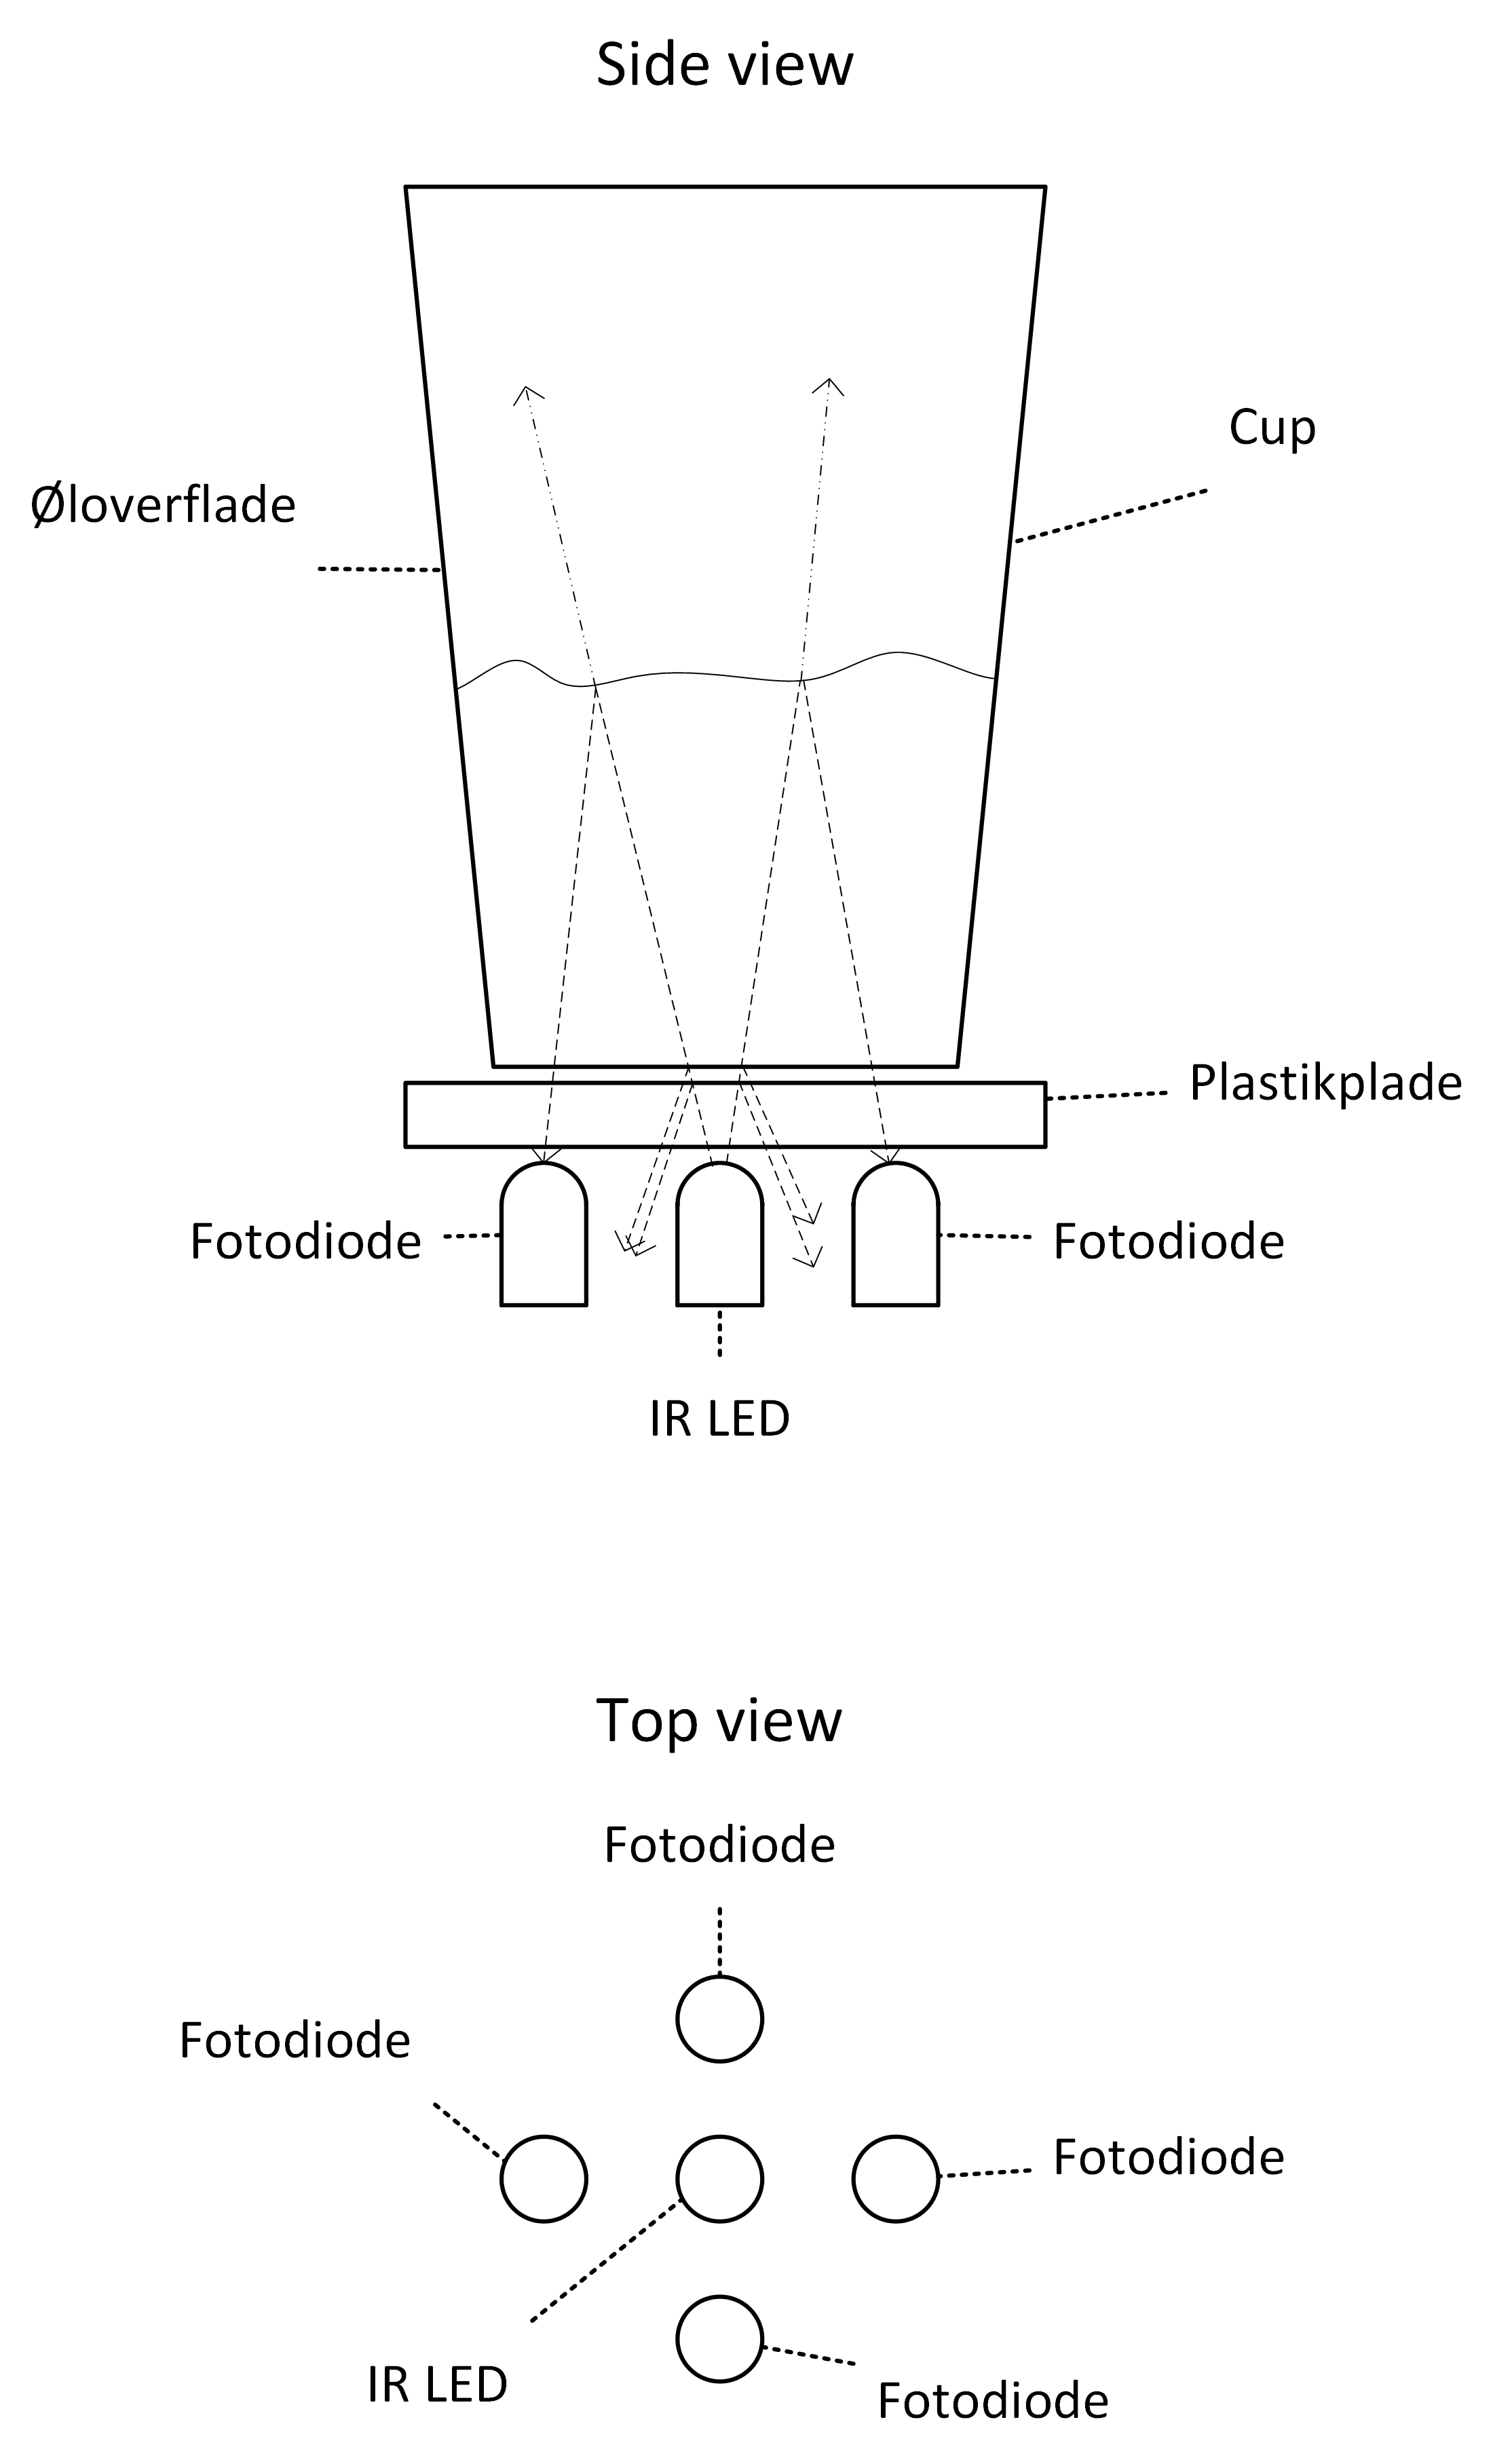
\includegraphics[width=0.8\textwidth]{HardwareDesign/CupSensor/graphics/lightPath.png}
    \caption{Her ses hvordan opstillingen af sensoren skal være. Både fra siden og fra toppen. Der benyttes én IR LED, og fire fotodioder. Der er derudover tegnet Cup med øl og gennemsigtig plastikplade på skitsen. Der er også påtegnet hvordan det tænkes lyset vil bevæge sig}
    \label{fig:lightPaht}
\end{figure}

\subsubsection{Fotodiode beskrivelse} \label{sec:photodiode_description}
Der vil nu beskrives virkemåden af fotodioder som er valgt til at detektere lys. En fotodiode fungerer som det ses på figur \ref{fig:photodiode_operation}. En fotodiode har den karakteristiske spænding-strøm forhold som en normal diode. Dette forhold ændres når fotodioden belyses. Her rykkes hele grafen ned, alt efter lysintensiteten. Der begynder altså at løbe en strøm i spærreretningen. Hvis spændingen over dioden holdes konstant vil strømmen der løber i spæreretningen afhænge af lysintensiteten. 
\begin{figure}[H]
    \centering
    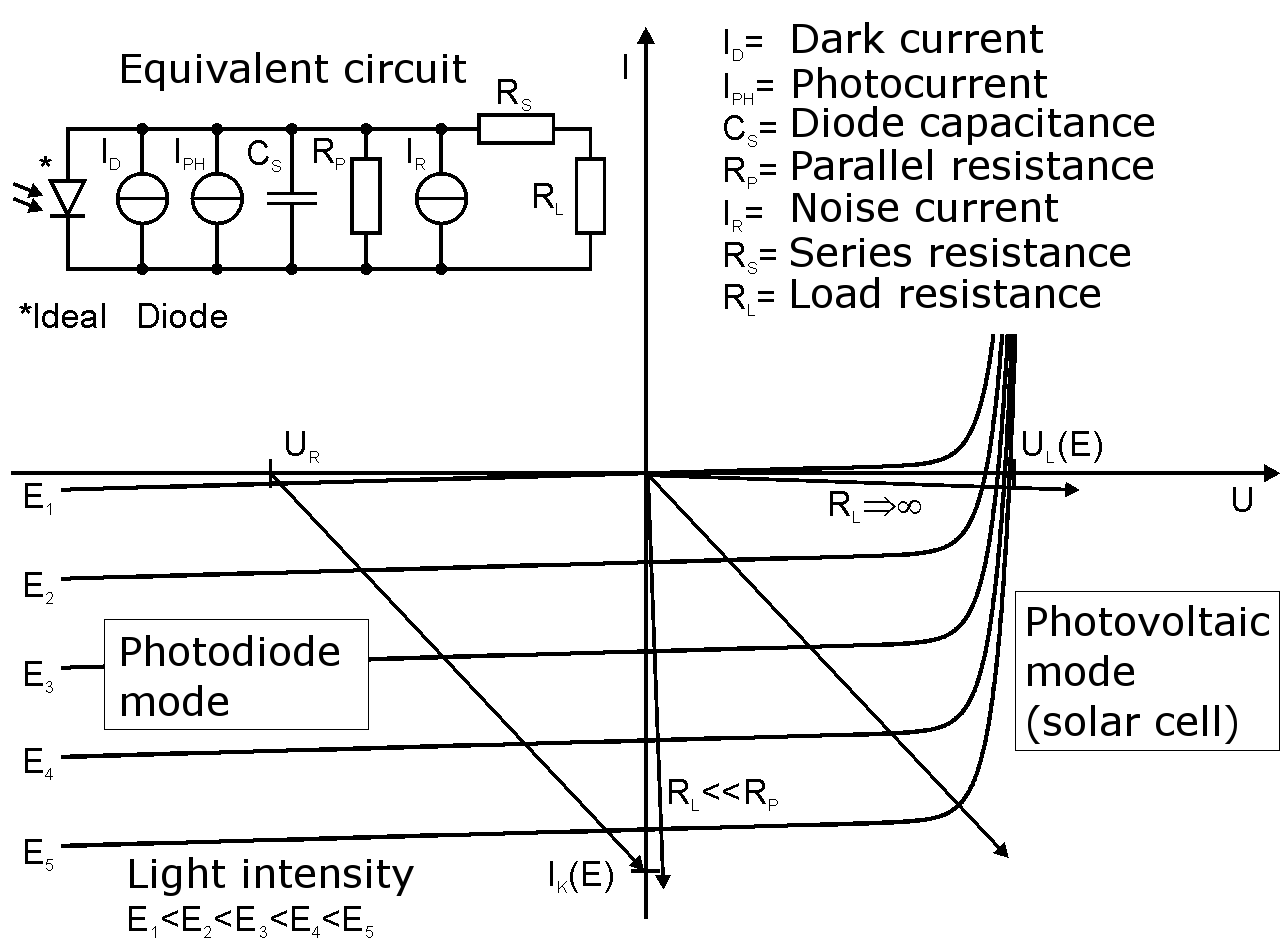
\includegraphics[width=\textwidth]{HardwareDesign/CupSensor/graphics/Photodiode_operation.png}
    \caption{Funktionalitet for en fotodiode \autocite{photodiodeWikipedia}}
    \label{fig:photodiode_operation}
\end{figure}

Til at benytte en fotodiode, ønskes en simpel model for en fotodiode. En model kunne være den som ses på figur \ref{fig:photodiodeModel}.

\begin{figure}[H]
    \centering
    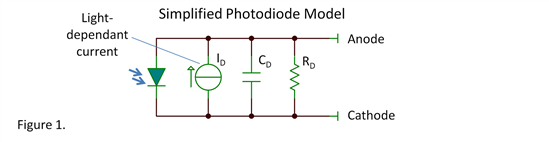
\includegraphics[width=\textwidth]{HardwareDesign/CupSensor/graphics/photodiodeModel.png}
    \caption{Model for fotodiode\autocite{photodiodesTI}}
    \label{fig:photodiodeModel}
\end{figure}

Det har ikke være muligt at finde tilstrækkelig oplysninger i databladet\autocite{SFH203FA} for den benyttede fotodiode til at benytte denne model. Fx er $R_D$ ikke angivet nogen steder. Det antages derfor at R\_D er så stor at den ikke har nogen betydning. Der benyttes i stedet en mere simpel model bestående kun af en strømkilde og en kondensator. som det ses på figur \ref{fig:photodiodeModelSimple}.

\begin{figure}[H]
    \centering
    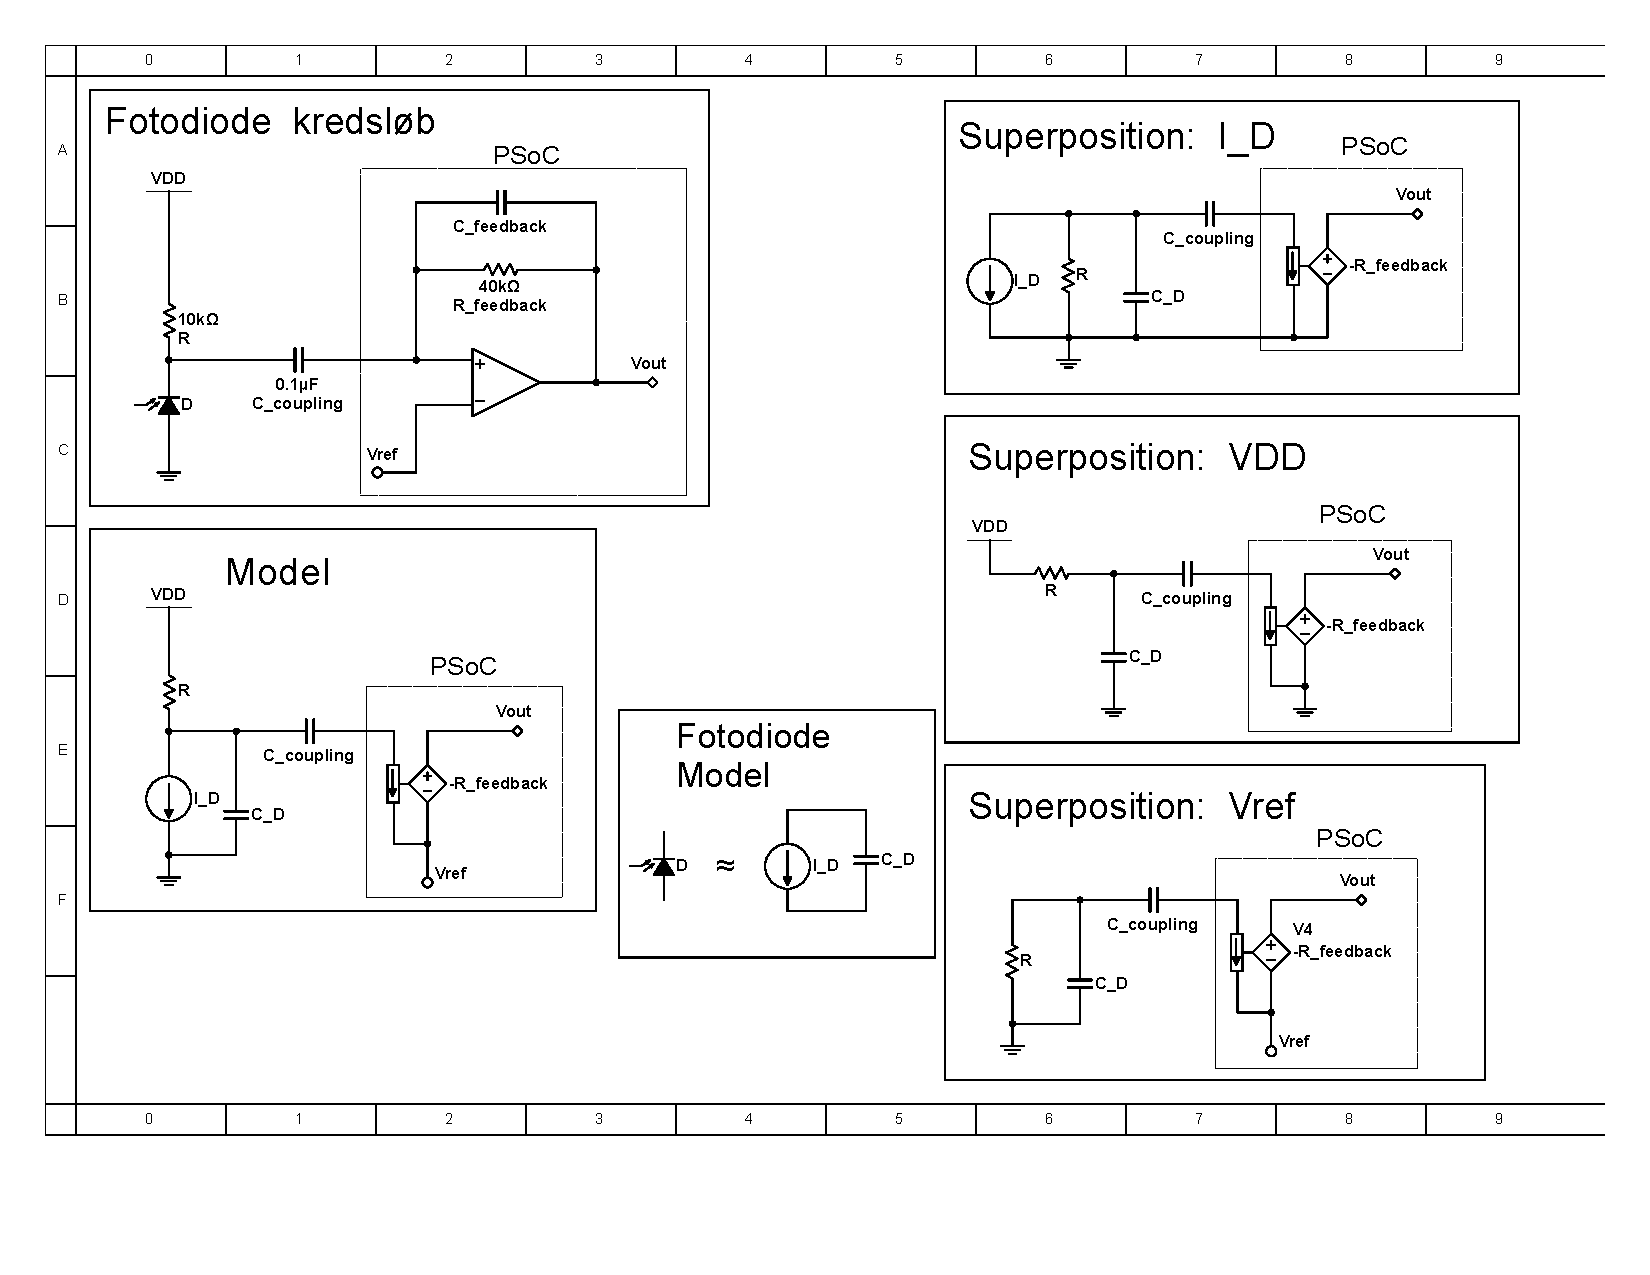
\includegraphics[width=0.9\textwidth,trim={4.1in 2.1in 4.75in 4.7in},clip, page=1]{HardwareDesign/CupSensor/graphics/Superposition.pdf}
    \caption{Anvendt model for fotodiode}
    \label{fig:photodiodeModelSimple}
\end{figure}

\subsubsection{AC kobling} \label{sec:CupSensorACCoupling}
Strømmen ønskes at laves om til en spænding. Men kun AC komponent af signalet, da LED'en blinker vil nyttesignalet være et AC signal. Der benyttes standard kredsløbet fra øvelse 6 i MSE\autocite{MSE_EXC_6}. Dette kan ses på figur \ref{fig:photodiodeCircuit}. Der benyttes ind til videre komponentværdierne som forslåes i øvelsesvejledningen.   DC komponenten af signalet filtreres væk vha. RC ledet. Den resterende AC strøm konverteres ligesom i teknologiundersøgelsen om til en spænding vha. en TIA. 
\begin{figure}[H]
    \centering
    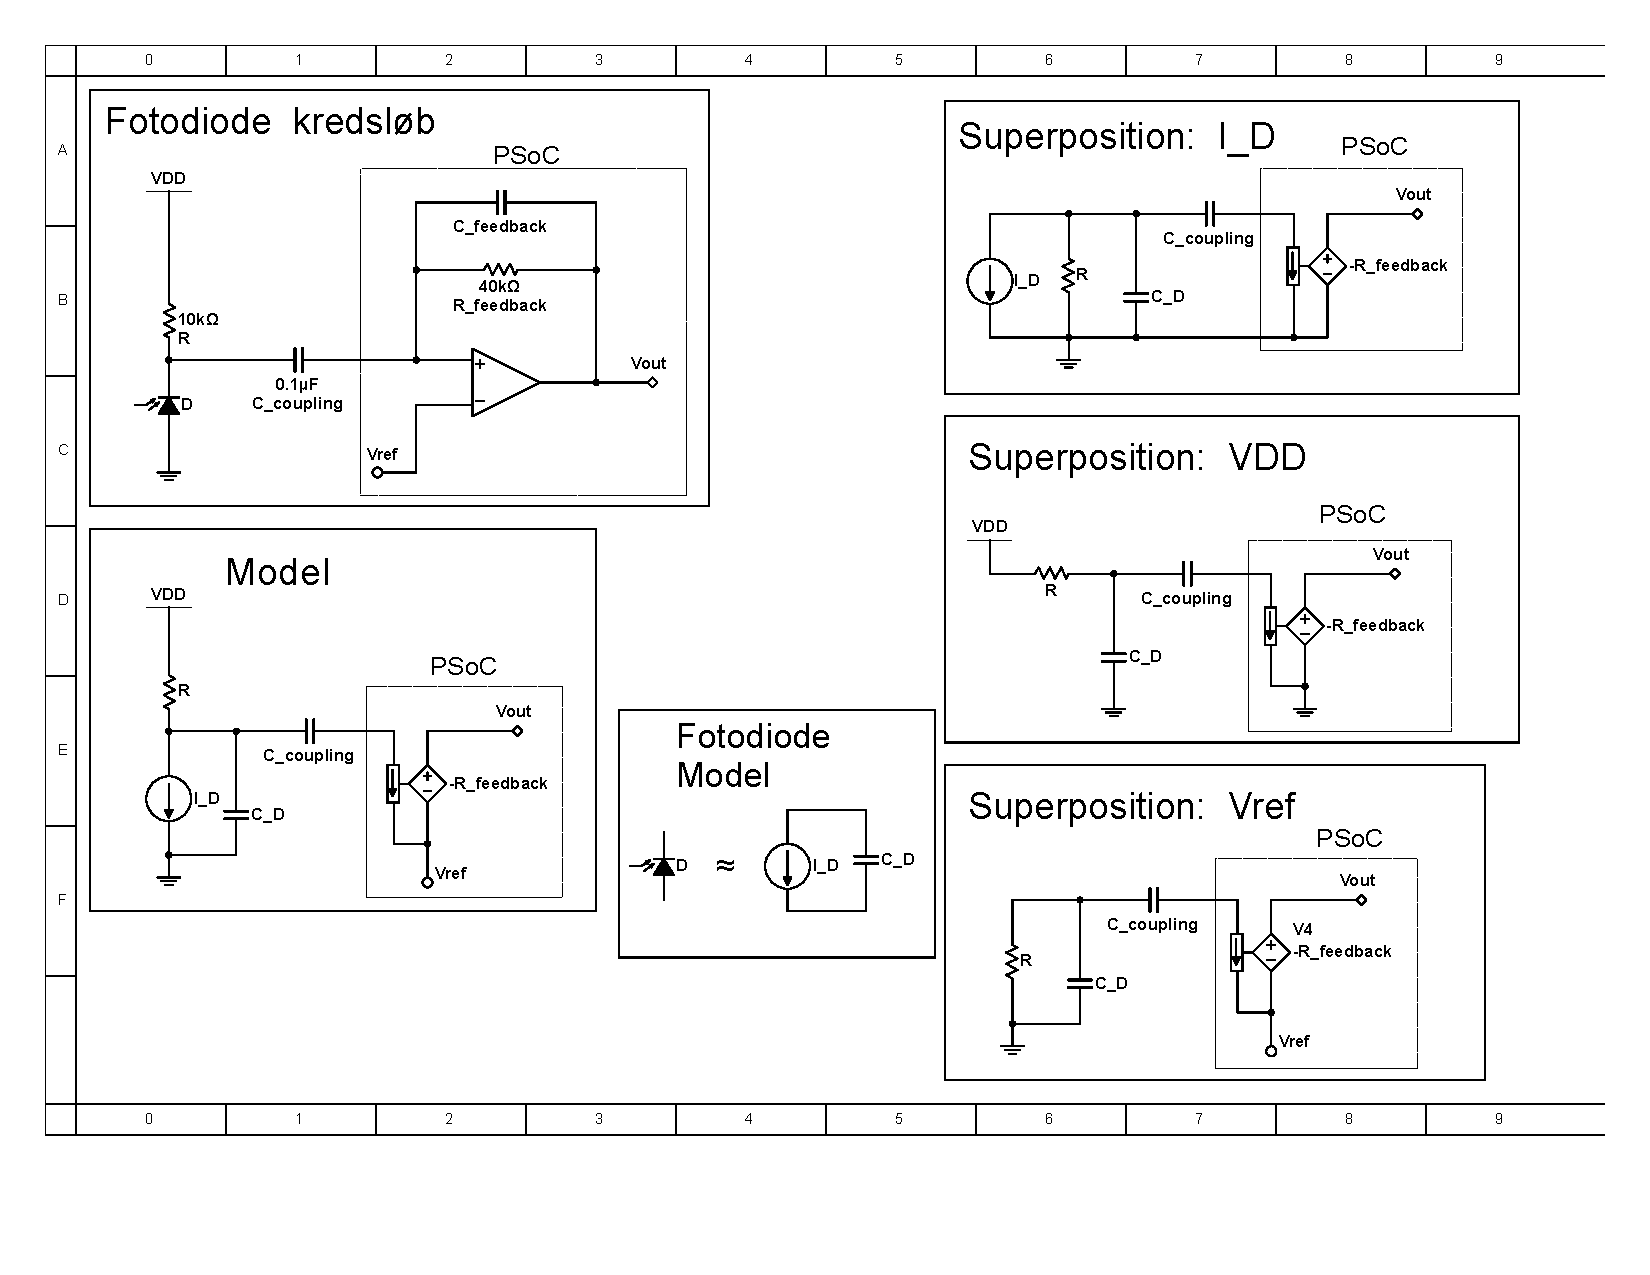
\includegraphics[width=0.9\textwidth,trim={0.6in 5.1in 6.0in 0.55in},clip, page=1]{HardwareDesign/CupSensor/graphics/Superposition.pdf}
    \caption{Diagram for fotodiode kredsløb}
    \label{fig:photodiodeCircuit}
\end{figure}
På \ref{fig:photodiodeCircuit} ses at der er en modstand R, som bl.a. sørger for at der hele tiden er påtrykt en spænding i spæreretningen. Dette er en af ændringerne i forhold til kredsløbet fra teknologiundersøgelsen. Spændingen i spæreretningen sørger for at formindske kondensatoren $C_D$ på figur \ref{fig:photodiodeModelSimple}. Det at kondensatoren formindskes kan ses ud fra databladet for SFH485 (se figur \ref{fig:CD-graph}).
\begin{figure}[H]
    \centering
    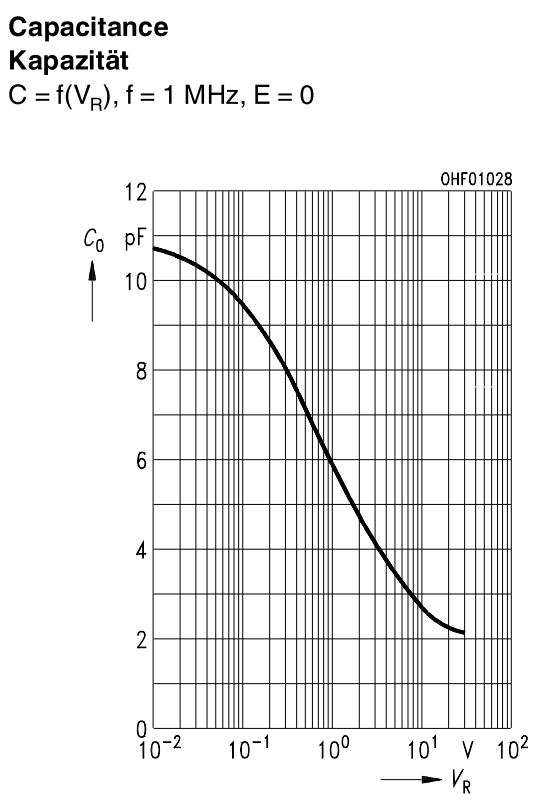
\includegraphics[width=0.9\textwidth]{HardwareDesign/CupSensor/graphics/CapacitancePhotodiode.PNG}
    \caption{Graf der viser fotodiodens kapacitet som funktion af spændingen i spæreretningen. Fra databladet for SFH203FA\autocite[6]{SFH203FA}}
    \label{fig:CD-graph}
\end{figure}
Det ses at $C_0$ (i vores model $C_D$) bliver mindre jo større $V_R$ er. $V_R$ er 'reverse voltage' og altså spændingen i spæreretningen. Ved at tilføje modstanden R, sørges der for at $V_R$ altid er positiv. Dermed er $C_0 = C_D \approx 3.5\si{pF}$ ved $V_R=5\si{V}$. Det ønskes at sænke kapacitansen for $C_D$ da dette vil øge båndbredden for dioden da kondensatoren ikke skal påføres så stor en ladning. Derudover påvirker en kondensator på indgangen af en operationforstærker også stabiliteten af denne operationsforstærker.

Kredsløbet fungerer på sådan en måde at det offset der vil være fra fotodioden, grundet mørkestrømmen (dark current) og lys fra omgivelserne, bliver filtreret fra vha. AC kobling kondensatoren $C_{coupling}$. Dette vil forklares vha. superposition. Men først laves en model for kredsløbet, i denne model indgår både modellen for dioden og en model for TIA benyttes, som er en strømstyret spændingskilde. Denne model kan ses på figur \ref{fig:photodiodeCircuitModel}. 
Da der er negativ feedback på operationsforstærkeren vil det svare til at den ikke-inverterende indgang har samme spænding som den inverterende indgang. Dette er også medtaget på modellen. Derudover er forstærkningen for den strømstyret spændingsforsyning $-R_{feedback}$. Det ses på diagrammet at strømmen som styre spændingen er strømmen igennem $C_{coupling}$. Denne strøm noteres $I_{coupling}$ og spændingen på den strømstyret spændingkilde er derfor$-R_{feedback} I_{coupling}$.

\begin{figure}[H]
    \centering
    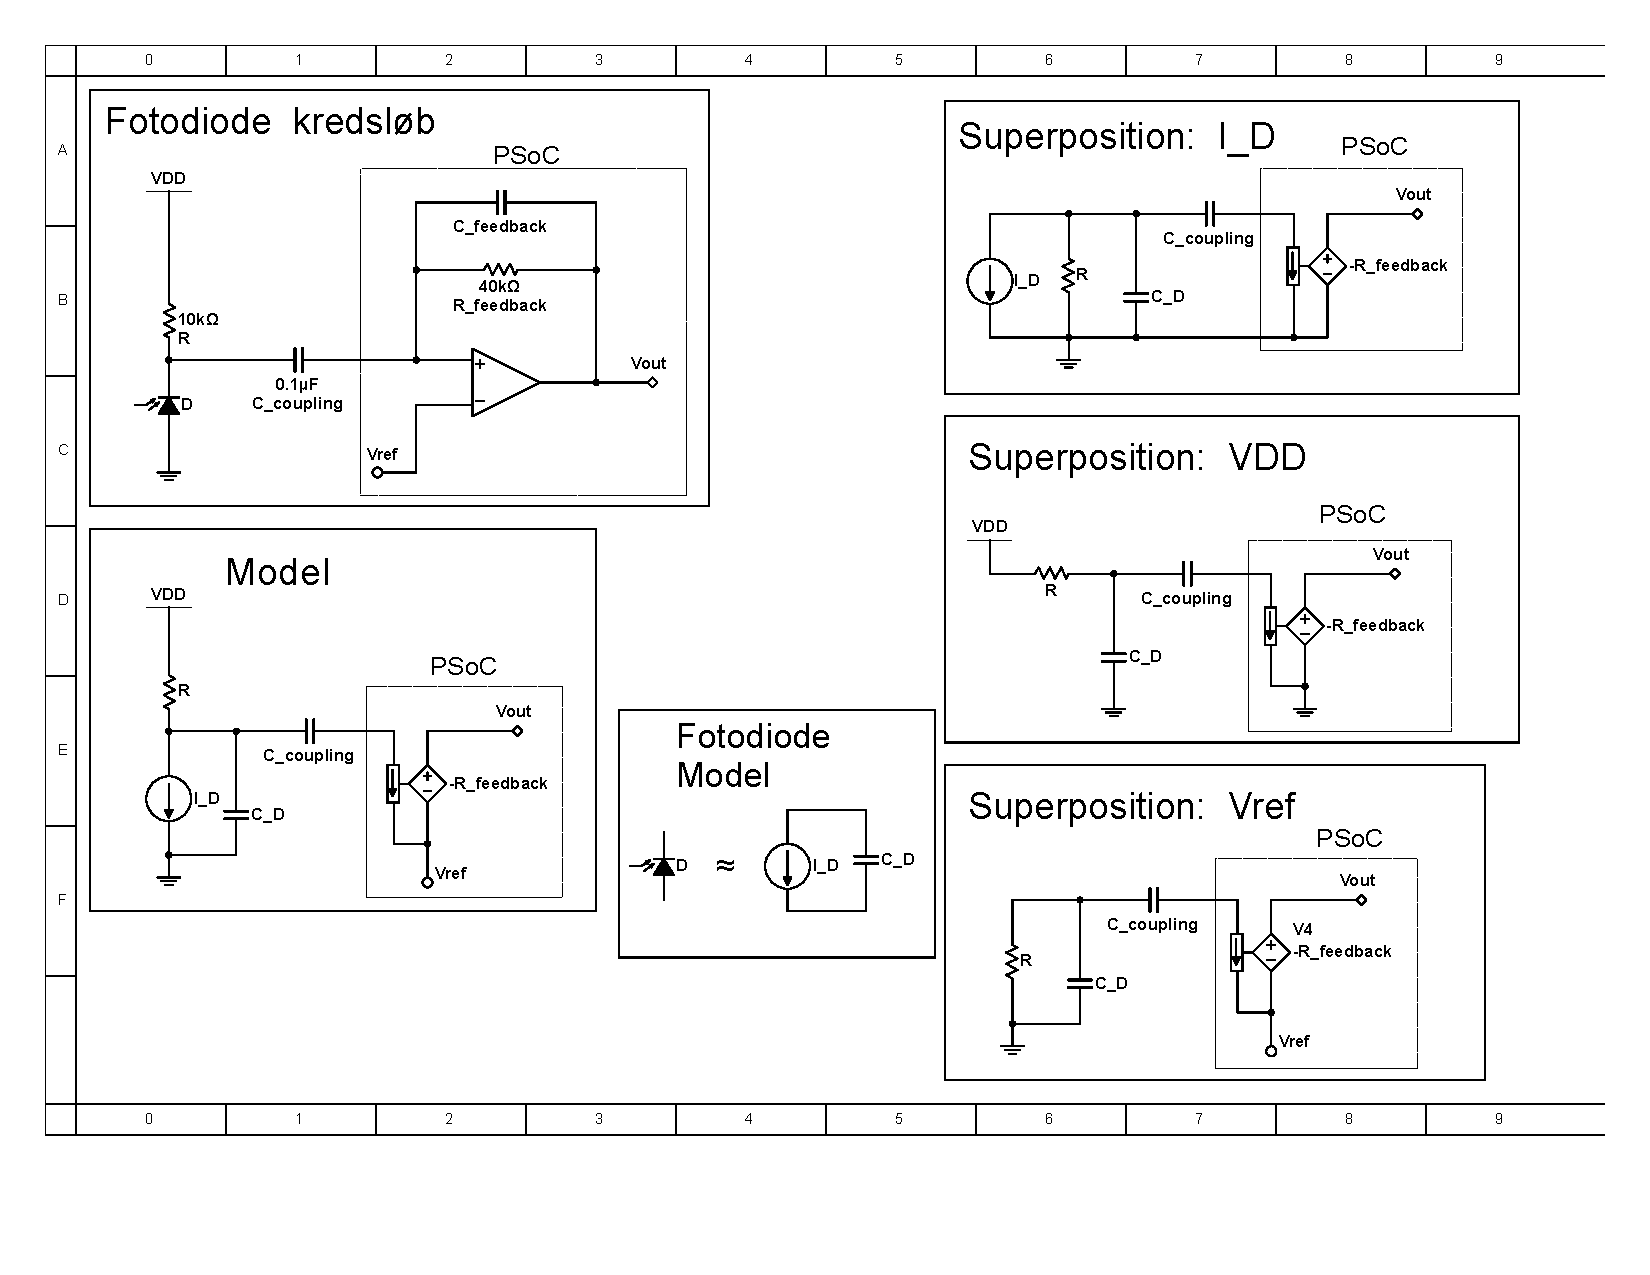
\includegraphics[width=0.9\textwidth,trim={0.6in 2.4in 7in 3.5in},clip, page=1]{HardwareDesign/CupSensor/graphics/Superposition.pdf}
    \caption{Model for fotodiode kredsløb}
    \label{fig:photodiodeCircuitModel}
\end{figure}

Der benyttes nu superposition hvor alle andre kilde end Vref slukkes (udover selvfølgelig den afhængige kilde). Til dette er der lavet et diagram som beskriver situationen, som kan ses på figur \ref{fig:photodiodeSPVref}. Der ses at $V_{ref}$ er forbundet til $C_{coupling}$, og da $V_{ref}$ er en DC spænding og en kondensator fungere som et åbent kredsløb ved DC, løber der derfor ikke nogen strøm ($I_{coupling\_Vref}=0$) og dermed er $V_{out\_Vref}=V_{ref}$ Der bruges notationen hvor Vref skrives i subscripten for at indikere at det er outputtet når kun $Vref$ er tændt.

\begin{figure}[H]
    \centering
    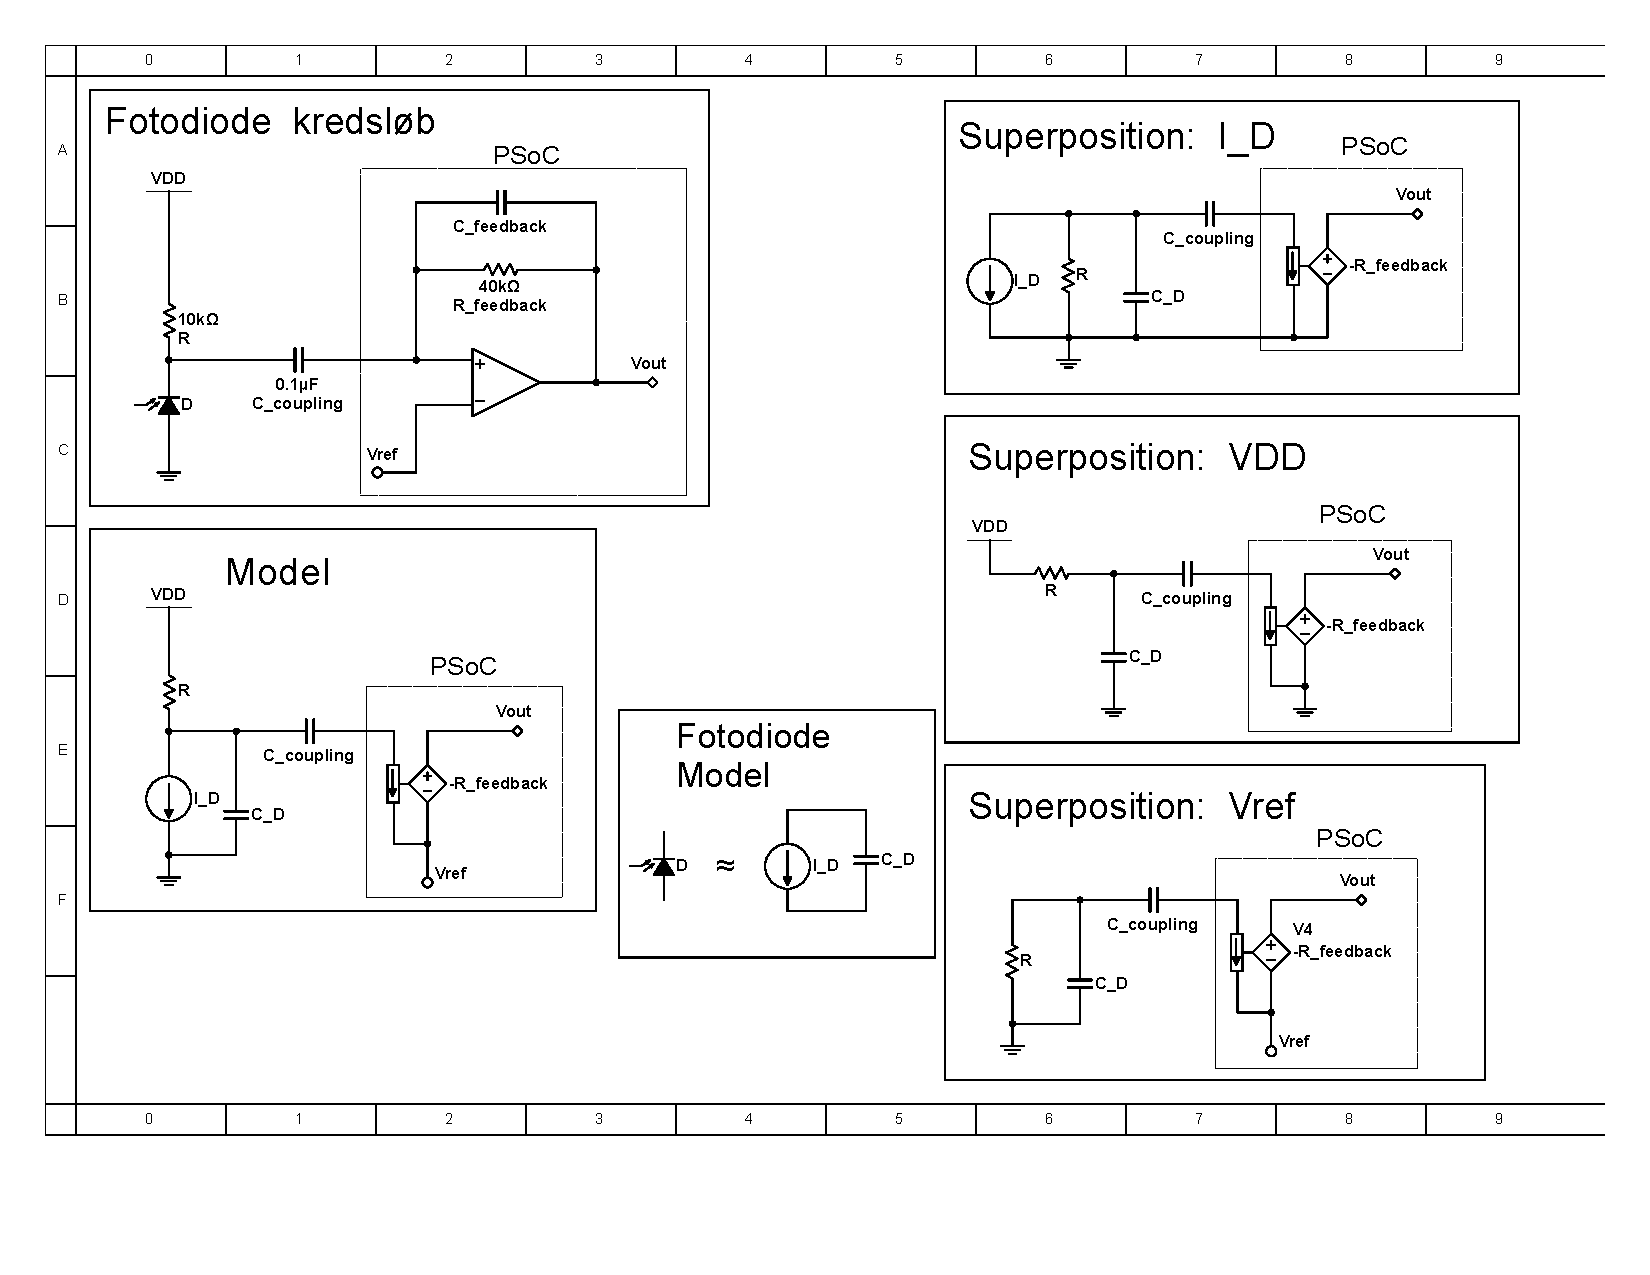
\includegraphics[width=0.9\textwidth,trim={6.3in 1.3in 1in 5in},clip, page=1]{HardwareDesign/CupSensor/graphics/Superposition.pdf}
    \caption{Fotodiode kredsløb når alle andre kilder end $Vref$ slukkes}
    \label{fig:photodiodeSPVref}
\end{figure}

Herefter benyttes superposition hvor kun VDD er tændt. Til dette er der lavet et digram som beskriver situationen, som kan ses på figur \ref{fig:photodiodeSPVDD}. Der ses igen at VDD er forbundet til $C_{coupling}$ og ligesom før, løber der ingen strøm igennem den ($I_{coupling\_VDD}=0$). Dermed er $V_{out\_VDD}=0$

\begin{figure}[H]
    \centering
    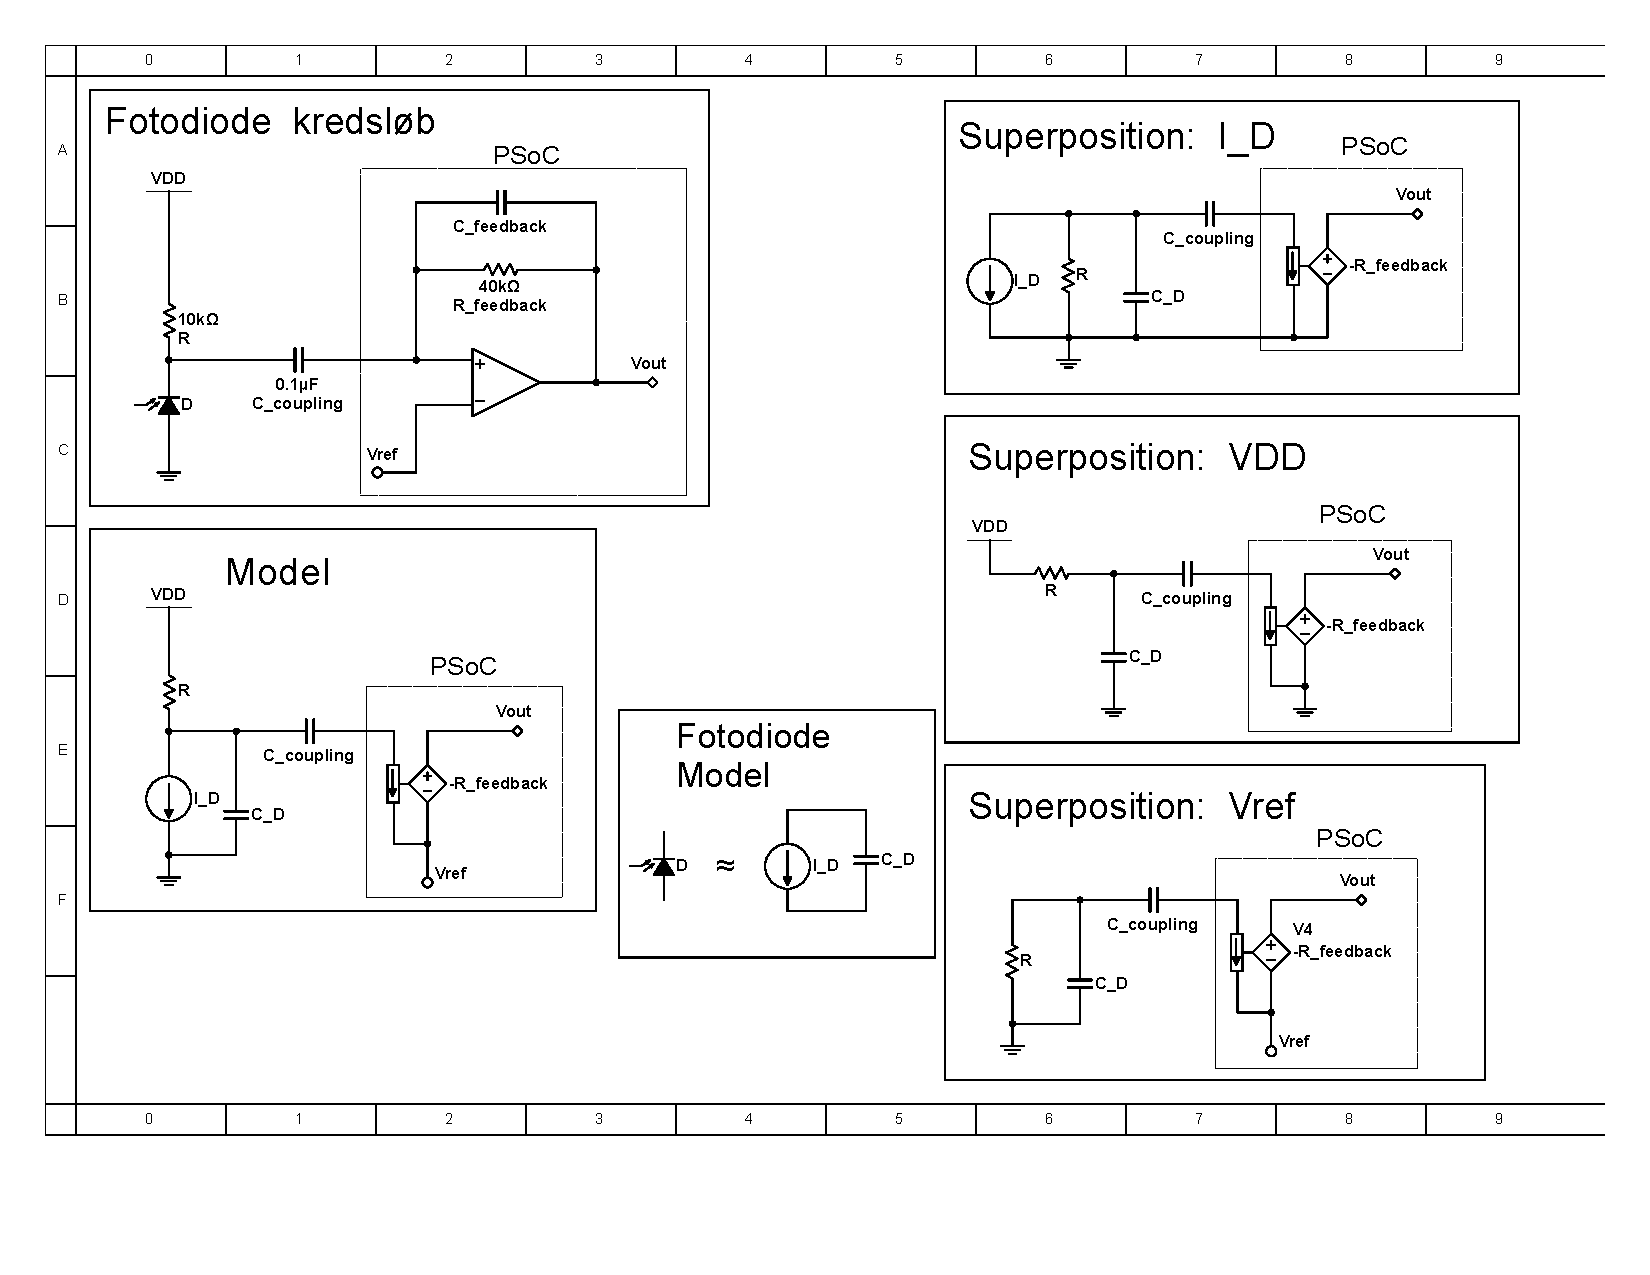
\includegraphics[width=0.9\textwidth,trim={6.3in 3.5in 0.8in 2.7in},clip, page=1]{HardwareDesign/CupSensor/graphics/Superposition.pdf}
    \caption{Fotodiode kredsløb når alle andre kilder end $VDD$ slukkes}
    \label{fig:photodiodeSPVDD}
\end{figure}

Til sidst undersøges situationen hvor kun $I_D$ er tændt. Til dette er der lavet et digram som beskriver situationen, som kan ses på figur \ref{fig:photodiodeSPI_D}. 

\begin{figure}[H]
    \centering
    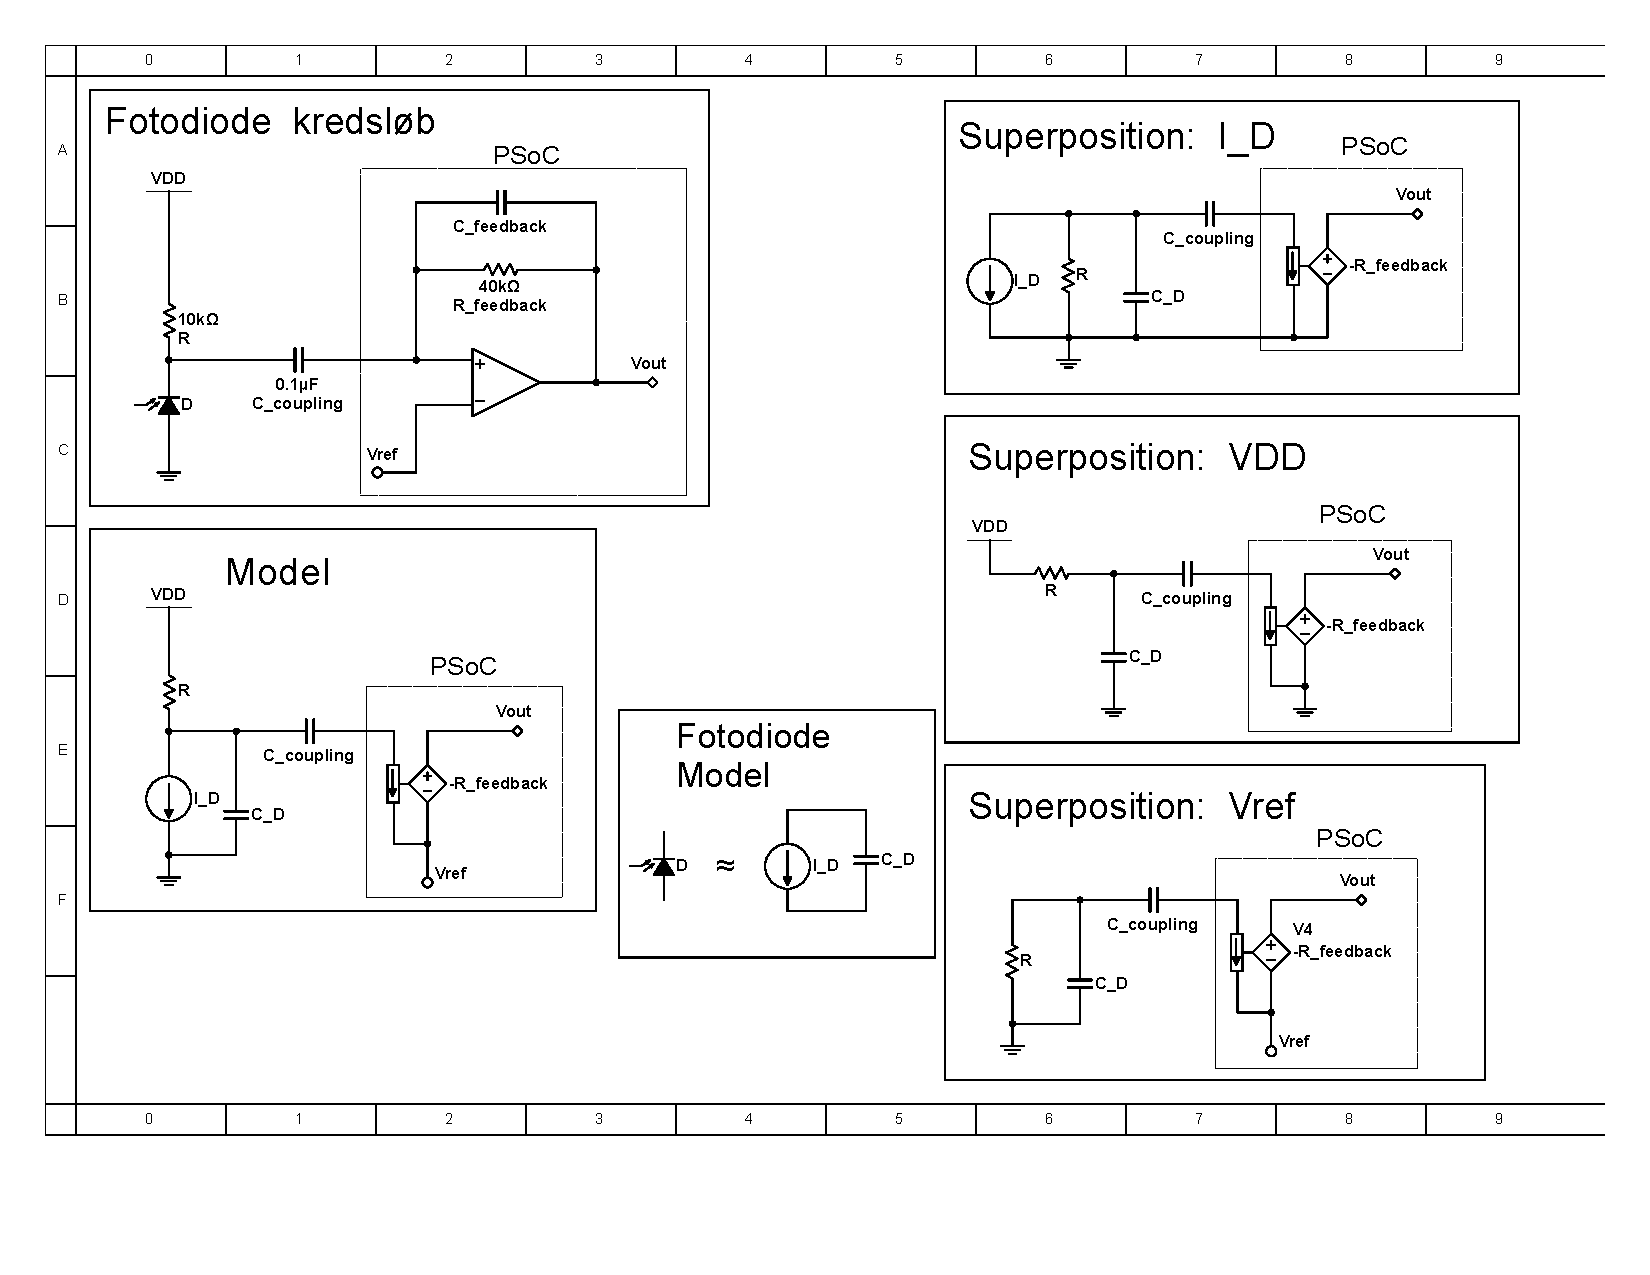
\includegraphics[width=0.9\textwidth,trim={6.3in 5.8in 0.8in 0.6in},clip, page=1]{HardwareDesign/CupSensor/graphics/Superposition.pdf}
    \caption{Fotodiode kredsløb når alle andre kilder end $VDD$ slukkes}
    \label{fig:photodiodeSPI_D}
\end{figure}

Der ses at der er en parallel kobling af de fire komponenter $I_D$, $R$, $C_D$ og $C_{coupling}$. Derfor kan strømmen $I_{coupling\_I\_D}$ bestemmes vha. strømdeling. 
$$
I_{coupling\_I\_D} = - I_D \frac{Y_{coupling}}{Y_R + Y_D + Y_{coupling}}
$$
hvor
$$
Y_R = \frac{1}{R} \textrm{,} \quad Y_D = C_D \dot s \quad \textrm{og} \quad Y_{coupling} = C_{coupling} s
$$
Dermed er strømmen
\begin{align}
I_{coupling\_I\_D} &= -I_D \frac{C_{coupling} s}{\frac{1}{R} + C_D s + C_{coupling} s}\\
&= - I_D \frac{R C_{coupling} s}{1 + R\left(C_D + C_{coupling} \right)s}\\
&=  - I_D \frac{\frac{R C_{coupling}}{R\left(C_D + C_{coupling} \right)} s}{\frac{1}{R\left(C_D + C_{coupling} \right)} + s}\\
&= - I_D \frac{C_{coupling}}{C_D + C_{coupling}} \frac{s}{\frac{1}{R\left(C_D + C_{coupling} \right)} + s}
\end{align}

Dermed er udgangen

\begin{align}
V_{out\_I\_D} &= -R_{feedback}I_{coupling\_I\_D}\\
&= I_D \frac{C_{coupling}R_{feedback}}{C_D + C_{coupling}} \frac{s}{\frac{1}{R\left(C_D + C_{coupling} \right)} + s}
\end{align}
Hvis $C_D << C_{coupling}$ kan det aproksimeres til
$$V_{out\_I\_D} = I_D R_{feedback} \frac{s}{\frac{1}{R C_{coupling}} + s}$$

Det ses at dette er et 1. ordens højpasfilter med cutoff frekvensen 
\begin{align}
\omega_c &= \frac{1}{RC_{coupling} }\\
&= \frac{1}{10\si{k\Omega} \cdot 0.1\si{\mu F}}\\
&= 1000 \si{\frac{rad}{s}}\\
f_c &= 159 \si{Hz}
\end{align}

Ud fra superposition kan det konkluderes at så læge $VDD$ og $V_{ref}$ er konstante og $C_D << C_{coupling}$ vil der kun detekteres AC komponenten fra $I_D$ med et offset på $V_ref$. Eller udtryk som nedenfor.
$$V_{out} = I_D R_{feedback} \frac{s}{\frac{1}{R C_{coupling}} + s} + V_{ref}$$

Dette er tildels hvad der ønskes, da LED'en blinker skal der kun detekteres AC komponenten fra fotodioden. Men det ønskes kun at detektere den del af signalet som har samme frekvens som LED'en blinker med. Til dette skal der laves et båndpas filter.

\subsubsection{Mixer}
Til at lave et båndpas filter er det valgt at benytte en mixer hvor lokaloscillatoren (LO) er den samme oscillator som styrer LED'en, dvs. samme frekvens og fase. 

Når der benyttes samme clock til at styre LED og til LO, er udgangen fra mixeren et DC niveau, når der ikke er støjsignaler tilstede. Herefter skal der benyttes et lavpasfilter som sammen med mixeren vil fungere som et båndpasfilter.

\newpage
\subsection{Håndtering af flere sensorer}

Der overvejes forskellige metoder til at håndtere flere sensorer.
\subsubsection{Flere kanaler}
Det overvejes at have én kanal til hver sensor. Et udkast til sådan en løsning kan ses på \ref{fig:multiple_channels}. Det vil sige at LED'erne på de forskellige sensorer (LED1 og LED2) blinker med forskellige frekvenser (Clock\_1 og Clock\_2). På denne måde kan man indstille kanalen på mixeren til den kanal der passer til den sensor der ønskes at blive læst. Dette gøres ved at indstille den lokale oscillator til mixeren (Clock\_3). Hvis det ønskes at læse fra sensoren bestående af LED1 og D1 indstilles Clock\_3 til at have samme frekvens som Clock\_1 (i eksemplet 11kHz). Denne løsning vil betyde at alle fotodioderne fra alle sensorerne kan forbindes til det samme ben på PSoC'en, hvilket er fordelagtigt.

\begin{figure}[H]
    \centering
    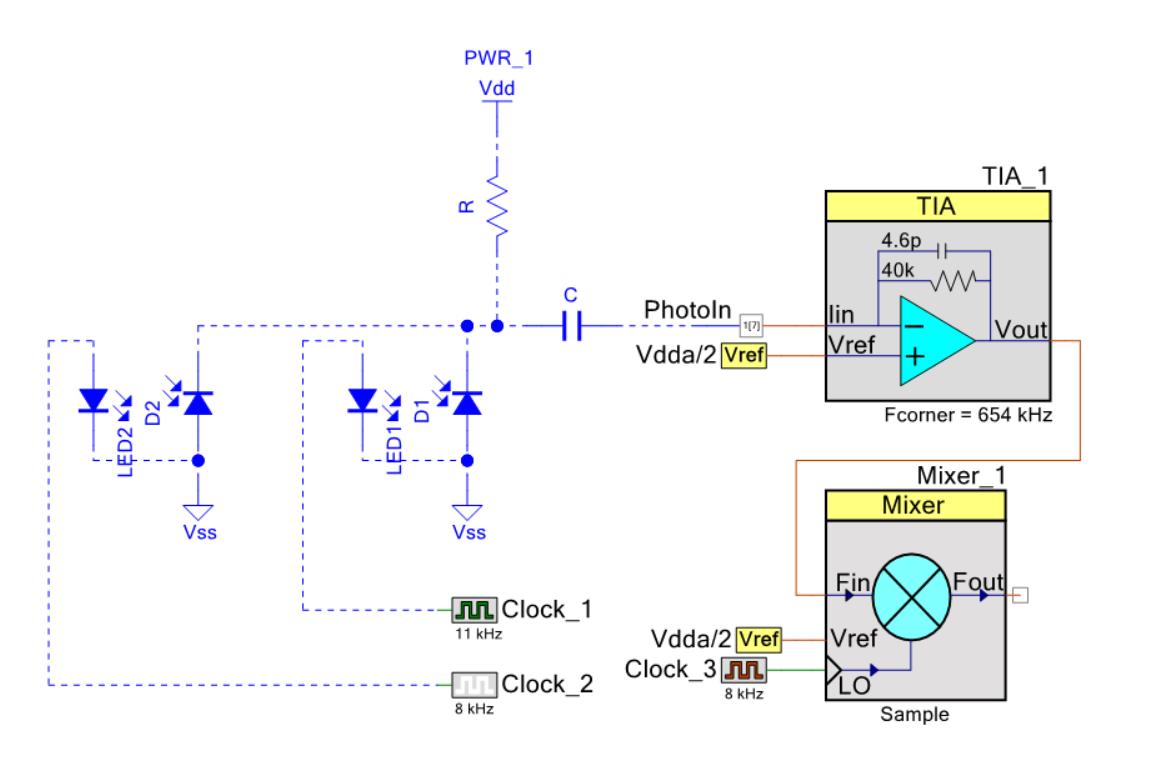
\includegraphics[width=1\textwidth]{HardwareDesign/CupSensor/graphics/Flere_kanaler.PNG}
    \caption{Udkast til hvordan kredsløbet kan se ud hvis der benyttes flere kanaler. Der er kun medtaget to sensorer(LED1 og D1 og den anden sensor er LED2 og D2). Der er for overskuelighedens skyld kun en fotodiode per sensor}
    \label{fig:multiple_channels}
\end{figure}

 En ulempe ved denne metode er, at TIA'en skal have en relativ lav forstærkning, for at den ikke går i mætning i de tilfælde hvor LED'en på alle sensorer er tændt på samme tid. Udgangen på mixeren vil være relativt lav da det jo kun er er fra en sensor. Der vil derfor kræves yderligere forstærkning på udgangen af mixeren. Hvis TIA'en derimod er indstillet til at forstærke signalet fra kun én sensor (som i de andre metoder beskrevet), kan denne forstærkning være ca 6 gange større.
 
 En fordel ved denne metode er at klok-signalet til hver sensor ikke nødvendigvis behøver at være på PSoC'en, man kunne have et lokalt kloksignal ved hver sensor for at minere brugen af ben på PSoC'en.

\subsubsection{Multiplexing}
En anden metode til at håndtere flere sensorer, er kun at sende kloksignalet til LED'en på én sensor af gangen og samtidig kun måle signalet fra fotodioderne på én sensor af gangen. Et udkast til sådan en løsning kan ses på \ref{fig:multiplexing}. Til dette skal der bruges 6 digitale udgange og 6 analoge indgange og tilsammen 12 ben på PSoC'en. Dette er en af ulemperne med denne løsning. Der ses på \ref{fig:multiplexing} at der benyttes en multiplexer og en de-multilexer til at sende kloksignalet til en sensor og kun at modtage fra en sensor. Multiplexeren og de-multiplexeren skal således styres sammen, så der læses signalet fra den samme sensor som der sendes et signal til.

\begin{figure}[H]
    \centering
    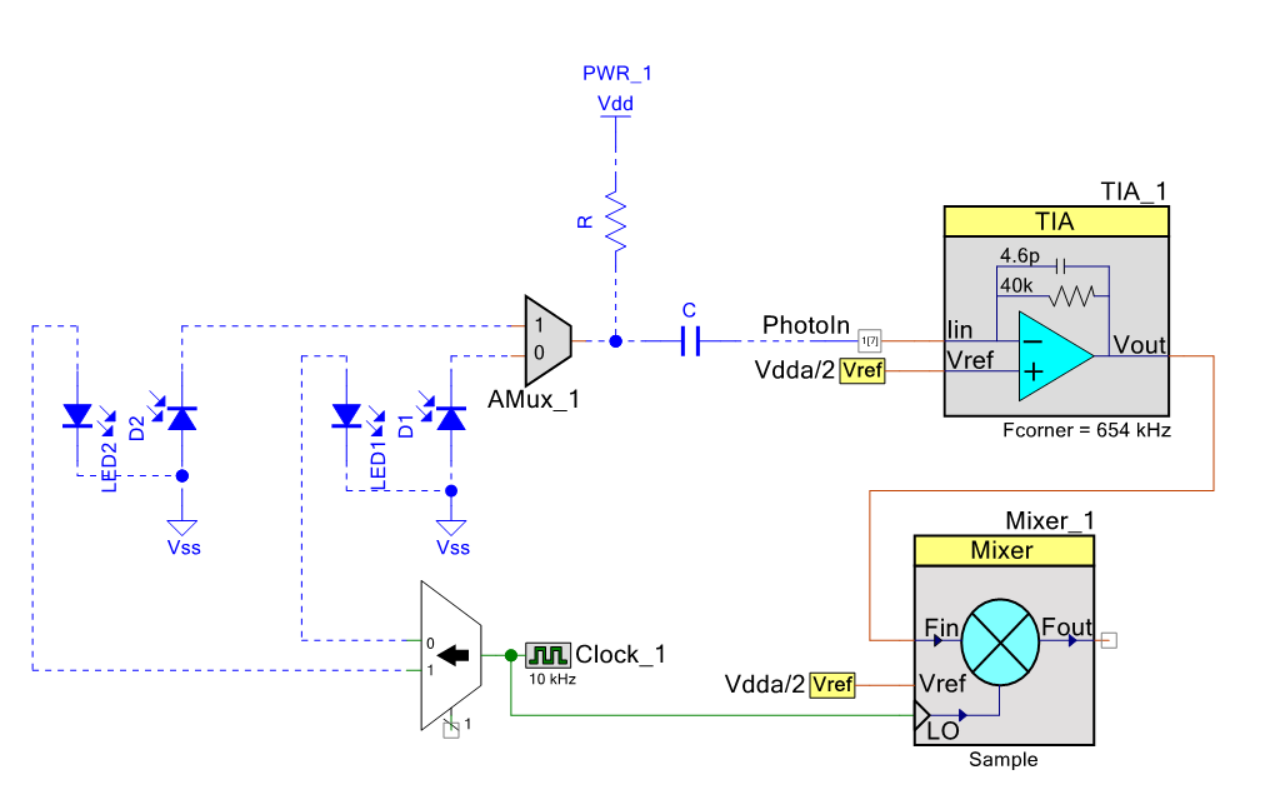
\includegraphics[width=1\textwidth]{HardwareDesign/CupSensor/graphics/Multiplexing.PNG}
    \caption{Udkast til hvordan kredsløbet kan se ud hvis der benyttes multiplexing. Der er kun medtaget to sensorer(LED1 og D1 og den anden sensor er LED2 og D2). Der er for overskuelighedens skyld kun en fotodiode per sensor}
    \label{fig:multiplexing}
\end{figure}

\subsubsection{Multiplexing med kun en indgang}
Der overvejes en anden variation af multiplexing. Et udkast til sådan en løsning kan ses på \ref{fig:multiplexing_en_indgang}. Der sendes stadig kloksignal til en sensor af gangen, men alle sensorers fotodioder forbindes til den samme analoge indgang på PSoC'en. Her vil det blive antaget at lyset der bliver sendt ud fra en sensor ikke påvirker fotodioderne på de andre sensorer. Hvis denne antagelse er gyldig kan alle sensorer måles men med færre ben på PSoC'en end den tideligere beskrevet multiplexing metode. En ulempe til denne metode er at antagelsen om at de andre fotodioder ikke bliver påvirket, muligvis ikke er gyldig.

\begin{figure}[H]
    \centering
    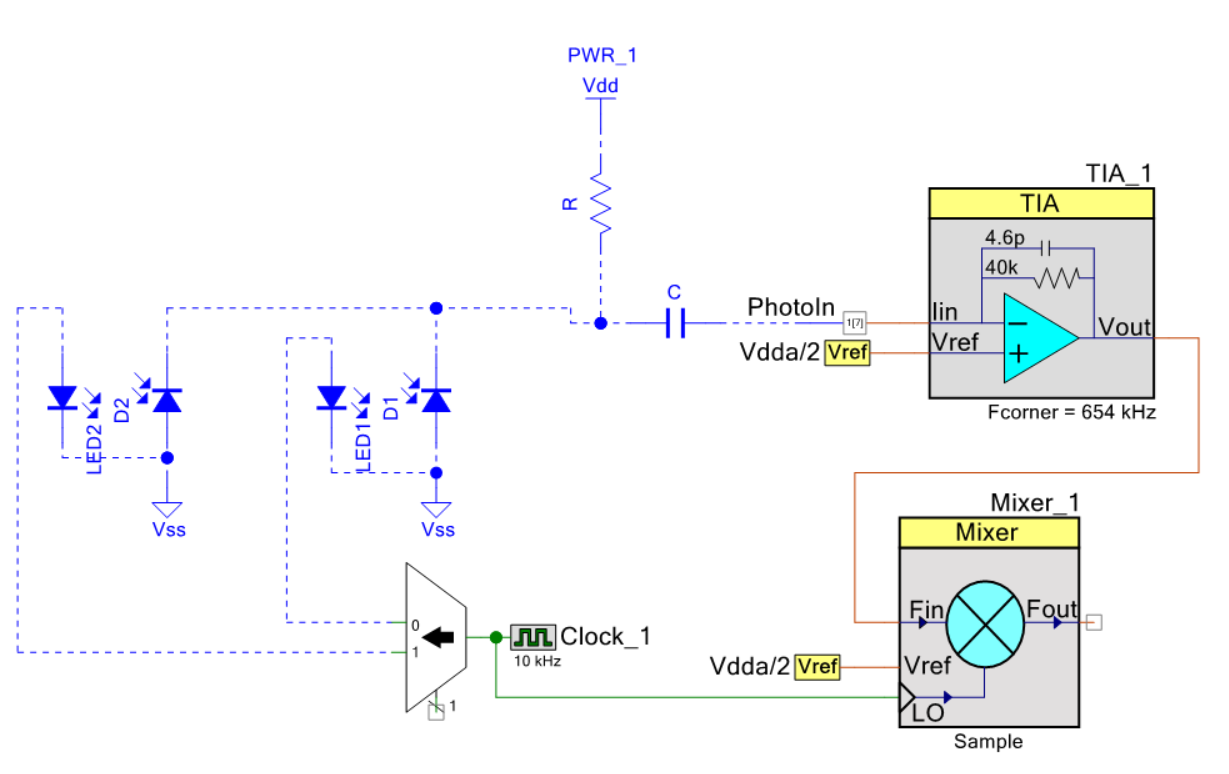
\includegraphics[width=1\textwidth]{HardwareDesign/CupSensor/graphics/Multiplexing_en_indgang.PNG}
    \caption{Udkast til hvordan kredsløbet kan se ud hvis der benyttes multiplexing med kun en indgang. Der er kun medtaget to sensorer(LED1 og D1 og den anden sensor er LED2 og D2). Der er for overskuelighedens skyld kun en fotodiode per sensor}
    \label{fig:multiplexing_en_indgang}
\end{figure}


\subsubsection{Udvidelse til Multiplexing med kun en indgang}
Der overvejes en udvidelse af multiplexing med kun en indgang. I denne udgave vil det kloksignal der sendes til LED'en på en sensor også styre om fotodiodernes strøm skal sendes videre til TIA'en. Så der kun modtages et signal fra den sensor der læses. En ulempe for denne metode er at der skal benyttes flere komponenter end tidligere metode, og systemet bliver mere kompliceret. En fordel er at det ikke er nødvendigt at antage at de andre fotodioder ikke bliver påvirket, da de ikke vil sende signalet videre til TIA'en, og det bliver derfor mere pålidligt.

\subsubsection{Valg af metode}
Det vil umiddelbart være bedst at benytte den metode hvor der er én kanal til hver sensor, da det fx. kunne være muligt at have en oscillator til hver sensor ekstern fra PSoC'en, så der kun skal bruges ét ben på PSoC'en. Der er med denne metode problemet at forstærkningen vil være lille og signalet på udgangen af mixeren derfor vil være relativt lavt (dette kan dog forstærkes op). Derudover skal der benyttes flere forskellige kloksignaler på PSoC'en hvilket vil benytte flere recourcer på PSoC'en. Denne metode fravælges derfor. 

Den simple metode med multiplexing (6 udgange og 6 indgange) vil være relativ nem at implementere (i forhold til nogle af de andre metoder) og nok også rimelig pålidelig. Dette er en meget god grund til at vælge denne metode, men den bruger mange ben. Selvom det ikke er noget direkte krav hvor mange ben der må bruges, så er det overordnet i projektet et ønske (ikke beskrevet nogen steder) at benytte så få ben som muligt, da det vil muliggøre at benytte en mindre microcontroller/PSoC i et endeligt produkt (De PSoC kits der bruges i dette projekt, tænkes at blive erstattet af en billigere og mindre microcontroller/PSoC). Derfor fravælges denne metode også.

Til sidst er der de to metoder med multiplexing hvor der kun benyttes en indgang. Disse metoder benytte færre ben end den simple multiplexing metode. Der bruges 7 ben frem for 12. Samme antal ben som der vil bruges med metoden med flere kanaler. Derfor vælges en af disse metoder (en af multiplexing metoderne med kun en indgang). Forskellen mellem de to metoder er hovedsageligt at den ene metode bygger på antagelsen om at lys udsendt fra én sensor, ikke vil påvirke fotodioderne på de andre sensorer. Derfor vælges det at arbejde videre med den metode hvor det antages at denne antagelse er gyldig, og hvis det viser sig at den ikke er, kan det overvejes at skifte til den anden metode.
\newpage
\subsection{Endeligt design} \label{sec:CupSensorFinalDesign}
Ud fra de tidligere afsnit er der udviklet udviklet et system. Hele designet fremgår på tre diagrammer. Diagrammer kan ses på figur \ref{fig:CupSensorDesign}, \ref{fig:CupSensorCupHolderControllerPart} og \ref{fig:CupSensorPSoCDesign}.

På figur \ref{fig:CupSensorDesign} er der en IR LED, som styres af en transistor. Der til LED'en en formodstand som er delt op i to for at kunne afsætte nok effekt. Der er fire fotodioder. De er alle i parallel. De er i parallel da fotodioderne fungerer som strømkilder, og strømmene fra hver fotodiode adderes derfor sammen, som løber i sensorOutput.
\begin{figure}[H]
    \centering
    \makebox[\textwidth][c]{%
        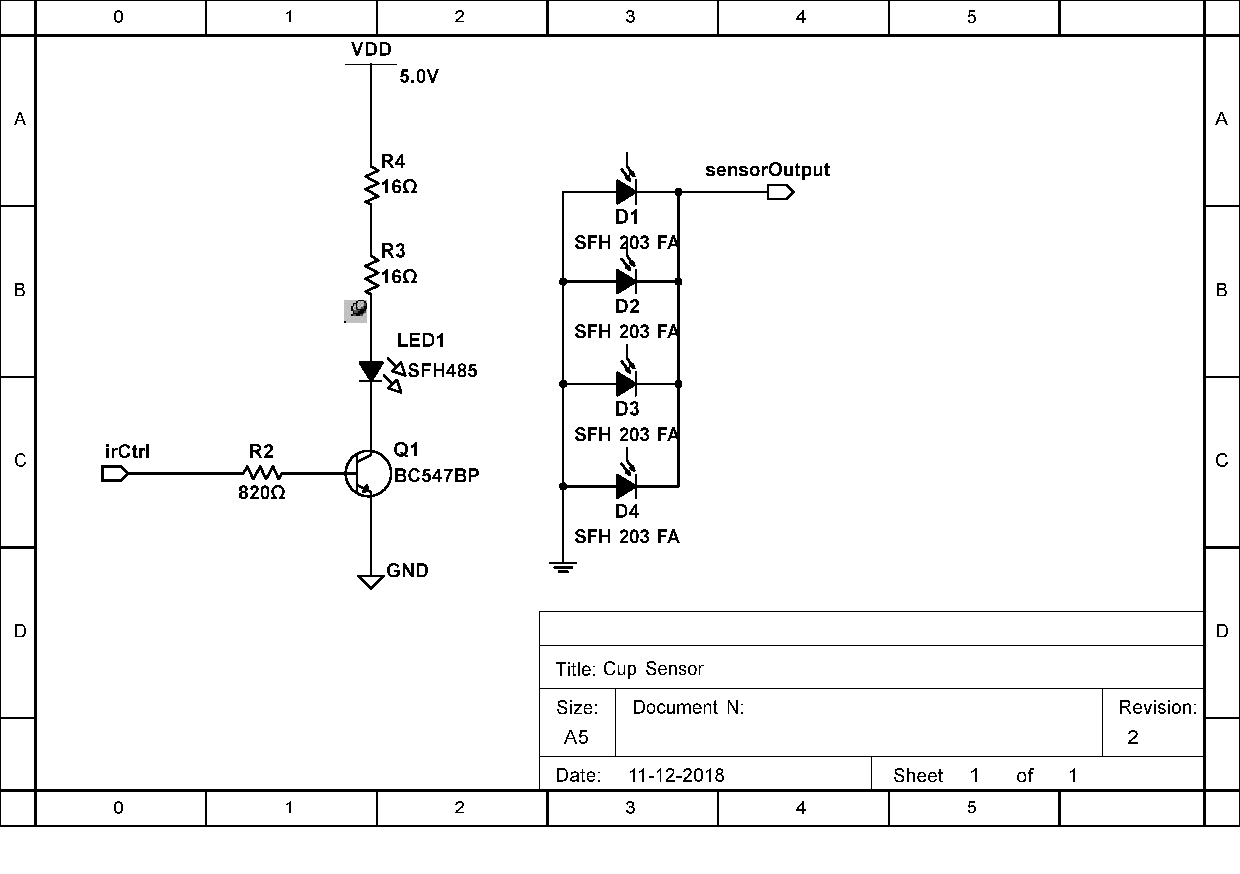
\includegraphics[width=1\columnwidth,trim={0.6in 1.8in 2.6in 0.25in},clip, page=1]{HardwareDesign/CupSensor/graphics/FinalDesign/CupSensor.pdf}
    }
    \caption{Design af Cup Sensor blokken}
    \label{fig:CupSensorDesign}
\end{figure}

På figur \ref{fig:CupSensorCupHolderControllerPart} er delen som skal modtage signal fra alle Cup Sensors ind til sensors. Det er alle forbundet til hinanden så der tilsammen er 4x6=24 fotodioder i parallel. 
\begin{figure}[H]
    \centering
    \makebox[\textwidth][c]{%
        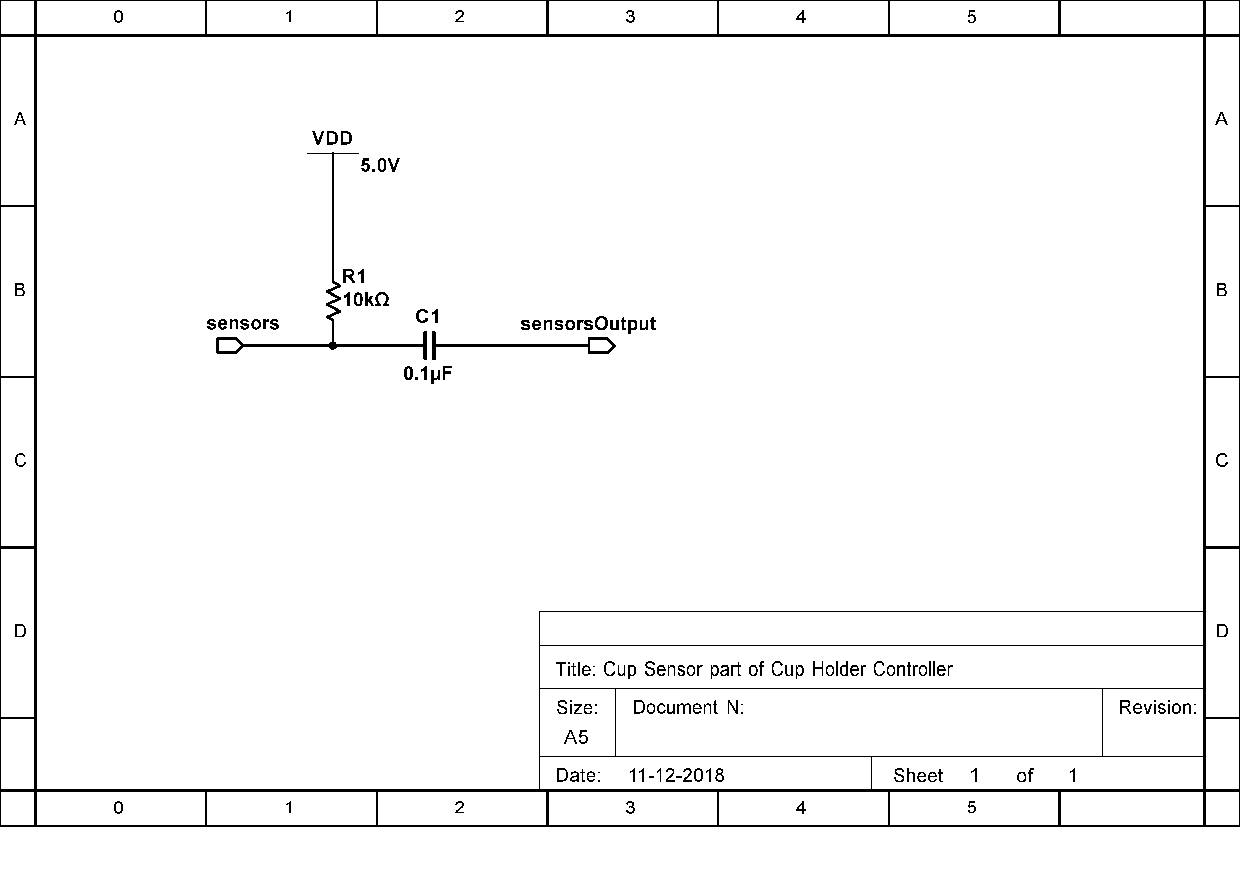
\includegraphics[width=0.7\columnwidth,trim={1.3in 3in 3.8in 0.5in},clip, page=1]{HardwareDesign/CupSensor/graphics/FinalDesign/CupSensorPart-CupHolderController.pdf}
    }
    \caption{Den del af Cup Holder Controller som sørger for at modtage signalet fra alle sensorer og filtrere DC fra.}
    \label{fig:CupSensorCupHolderControllerPart}
\end{figure}

På figur \ref{fig:CupSensorPSoCDesign} ses hardwaren komponenterne som der er på PSoC'en. Der er en TIA som konvertere strømmen sensorsOutput på figur \ref{fig:CupSensorCupHolderControllerPart} om til en spænding. Herefter er der en ADC som konvertere spændingen som samtidig har Mixer funktionalitet og filterfunktionalitet, som beskrives senere. Derefter er der en DMA som sørger for at flytte dataen fra ADC'en til hukommelsen i softwaren. Der er en demultiplexer som bruges til at styre hvilken Cup sensor der sendes et signal til at styre IR LED på Cup Sensor. Signalet der styres er et 10kHz firkant signal. Demultiplexeren styres af control registret Control\_Reg\_Led. Der er desuden en VDAC som bruges til at debugge systemet. Alle disse blokke er en del af en custom component \autocite{PSoCHowToCreateCustomComponents}.  i PSoC Creator 
\begin{figure}[H]
    \centering
    \makebox[\textwidth][c]{%
        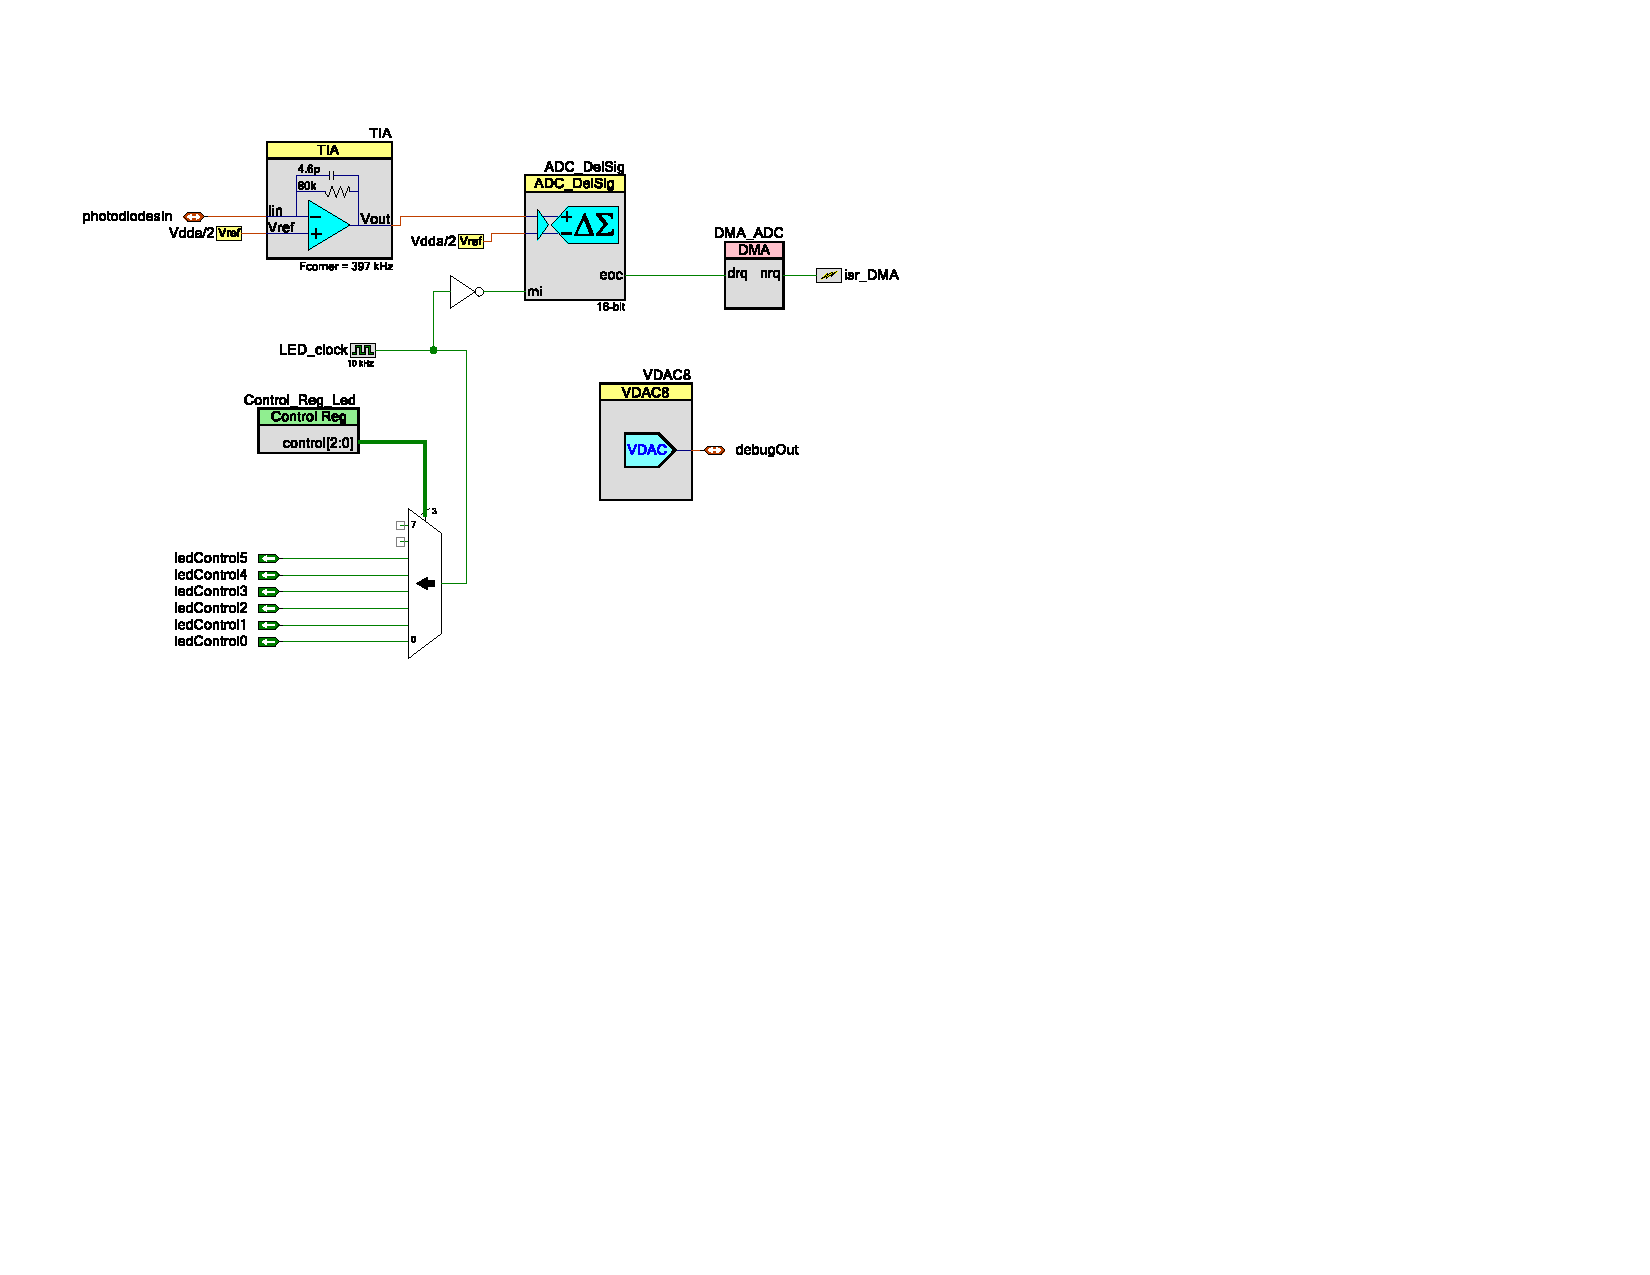
\includegraphics[width=1\columnwidth,trim={0.5in 4.1in 4.5in 0.8in},clip, page=1]{HardwareDesign/CupSensor/graphics/FinalDesign/PSoC-design.pdf}
    }
    \caption{PSoC design. 'photodiodesIn' forbindes til 'sensorsOutput' på figur \ref{fig:CupSensorCupHolderControllerPart}}
    \label{fig:CupSensorPSoCDesign}
\end{figure}

På figur \ref{fig:CupSensorComponentInTopDesign} ses custom komponent i brug i top design. Det eneste der udføres her er at forbinde de forskellige porte til fysiske porte på PSoC'en.   
\begin{figure}[H]
    \centering
    \includegraphics{}
    \caption{Den udviklede PSoC Custom komponent i brug i Top design}
    \label{fig:CupSensorComponentInTopDesign}
\end{figure}

\subsubsection{Valg af transistor}
Der skal benyttes en transistor til at styre LED1 på figur \ref{fig:CupSensorDesign}. LED1 kan håndtere en DC strøm på 100mA\autocite[7]{SFH485}. Den kan håndtere strømme på højere strømme ved en lav dutycycle og høj frekvens. Det er dog valgt at 100mA må være tilstrækkelig. Der blev som en del af teknologiundersøgelse benyttes 100mA, der der blev benyttes DC strømme. Det viste sig at være meget tilstrækkelig, det kan dog muligvis forbedre sensoren at øge strømmen, men det vælges ikke at gøre. 
Der skal derfor vælges en transistor som kan håndterer en strøm på 100mA. Det kan BC547 \autocite[2]{BC547}.

\subsubsection{Beregning af modstande}
De tre modstande på R2, R3 og R4 figur \ref{fig:CupSensorDesign} beregnes i dette afsnit. Basemodstanden R2 bestemmes nu. Transistoren skal gå i mætning og når transistoren er i mætning (conditions $I_C = 100\si{mA}, I_B = 5\si{mA}$) er $V_{BE}(sat)=900mV$\autocite[2]{BC547}. Da irCtrl er 5V logik er spændingen over modstanden derfor $V_{R2} = 5\si{V}-V_{BE}(sat)$
Værdien af modstanden skal derfor være $R2 = \frac{V_{R2}}{I_B}$. $I_B$ er ifølge de tidligere oplyste conditions $I_B = 5\si{mA}$.
$$R2=\frac{5\si{V} - 0.9\si{V}}{5\si{mA}} = 820\si{\Omega}$$

Formodstanden til LED1 bestemmes nu. Der løber en strøm på 100mA. Ifølge databladet for LED1, er spændingen over den $V_{LED1} = 1.5\si{V}$. Spændingen over transistoren er typisk $V_{CE}(sat) = 0.25\si{V}$. For modstanden til LED1 skal derfor være 
$$R_{LED} = \frac{V_{DD} - V_{LED1} - V_{CE}(sat)}{I_{LED}} = \frac{5\si{V}- 1.5\si{V} - 0.25\si{V}}{100\si{mA}} = 32.5\si{mA}$$
Der vil i modstanden blive afsat en effekt på $$I_{LED}^2 \cdot R_{LED} = \left(100\si{mA}\right)^2 \cdot 32.5\si{\Omega} = 325\si{mW}$$
De modstande der er tilrådighed kan kun afsætte $250\si{mW}$. Derfor vælges der at dele den modstanden op i to modstande på $16\si{\Omega}$.

\subsubsection{Mixer i ADC'en}
En ting der kan ses på diagrammet på figur \ref{CupSensorPSoCDesign} er, at der ikke er nogen mixer. Dette er fordi ADC'en har en indbygget funktion som kan få den til at have funktionaliteten af en mixer \autocite[3]{ADC-DelSig-datasheet}. Det er valgt da det formindsker antallet af nødvendige komponenter. ADC'ens mixer funktionalitet aktiveres ved at vælge "Enable modulator input" i konfigurationen af ADC'en. Når denne er valgt, har ADC'en inputtet 'mi'. Når dette input er højt, inverteres polariteten modulatoren i delta sigma ADC'en. På denne måde fungere ADC'en som en mixer, udover at en normal mixer vil invertere inputtet når LO er lav, derfor er der tilføjet en inverter mellem LED\_clock og 'mi' inputtet.

Formålet med at bruge en mixer er at lave et båndpasfilter. For at dette er tilfældet skal der på udgangen af mixeren være et lavpasfilter. Dette er også inkluderet i ADC'en som et sinc4 filter \autocite[35]{ADC_DelSig_datasheet}. Filteret virker som et lavpasfilter som vil have vil have uendelig stor dæmpning ved samplefrekvensen og alle dens harmoniske overtoner. Samplefrekvensen indstilles til 2500 samples/s. I kombination med mixeren vil det virke som et båndpas filter.  

\subsubsection{Fase forskydning}
Som tidligere beskrevet vil der på udgangen af en mixer være et DC niveau når det samme clocksignal bruges til styre lyset og lokaloscillatoren (LO) for mixeren. Men hvis de ikke er i fase kan man risikere at DC niveauet er nul. For at dette ikke sker, er det vigtigt at signalet til mixeren og LO har samme fase, eller tæ på samme fase. Det undersøges nu derfor om dette er tilfældet.

Det undersøges om lysets forsinkelse vil have en betydelig indflydelse på fasen af signalet fra fotodioden. Tidsforsinkelsen for lyset vil være 
$$t_d = \frac{l}{v_l}$$
hvor $t_d$ er tidsforsinkelse, $l$ er afstanden lyset bevæger sig og $v_l$ er hastigheden af lyset. Hvis det antages at hele den afstand, som lyset bevæger sig foregår i øl, som antages at være vand, er lysets hastighed $v_p = \frac{c}{n_{vand}}$, hvor $c$ er lysets hastighed i vakuum og $n_{vand}$ er brydningsindekset for vand.
Dermed er tidsforsinkelsen
$$t_d = n_{vand}\frac{l}{c}$$
fasen er dermed
$$\phi_{lys} = -2 \pi f_{LED\_clock} n_{vand}\frac{l}{c}$$, hvor $\phi_{lys}$ er fasen grundet lysets forsinkelse og $f_{LED\_clock}$ er frekvensen LED'en blinker med. Ved indsættelse af værdierne $n_{vand}=1.33$ \autocite{brydningsindex}, $f_{LED\_clock} = 10kHz$ og $l=1m$, som er meget længere end hvad det reelt vil være, fås fasen til 
$$\phi_{lys} = -0.032 \si{^{\circ}}$$

Det undersøges om AC koblingen vil have en betydelig indflydelse på fasen. I afsnit \fullref{sec:CupSensorACCoupling} blev nedenstående udtryk bestemt
$$V_{out\_I\_D} = I_D R_{feedback} \frac{s}{\frac{1}{R C_{coupling}} + s}$$
Dette udtryk gælder kun for når $C_D << C_{coupling}$ (hvor $C_D$ er kapaciteten af fotodioden og $C_{coupling}$ er C1) på figur \ref{fig:CupSensorCupHolderControllerPart}). Når der er 24 fotodioder i parallel, er $C_{D_{total}} = 24C_D =  24\cdot 3.5\si{pF} = 84\si{pF}$ Dette er når der er en spænding i spæreretningen. Da der kan løbe en relativ DC strøm i fotodioderne, som resultat af fx sollys, spændingen i værste tilfælde være 0V og så vil $C_D \approx 11\si{pF}$ og ud fra dette vil $C_{D_total} = 264\si{pF}$. I værste tilfælde vil $\frac{C_{coupling}}{C_{D_{total}}} = \frac{0.1\si{\mu F}}{264\si{pF}} \approx 378$. Så udtrykket kan stadig bruges, da $C_{D_{total}} << C_{coupling}$
Ved indsætningen af værdier for $R=10k\Omega$, $C_{coupling} = 0.1 \si{\mu F}$ og $s=j2\pi f_{LED\_clock} = j2\pi 10 \si{kHz}$ fås det at fasen er 
$$\phi_{ac\_kobling} = 0.912\si{^{\circ}}$$
Det kan konkluderes at der stort set ikke er nogen faseforskel. Den lille faseforskel der er, vil forårsage at DC niveauet vil være en lille smule mindre, men den vil være tæt på den maksimale mulige. 

\subsubsection{Signal conditioning}

\paragraph{Maksimal mulig signalstyrke}
{
For at bestemme TIA'ens forstærkning måles signalet fra TIA'en ved forskellige testscenarier. Signalet måles med den højeste feedbackmodstand på TIA'en uden at forstærkeren går i mætning. Fx går forstærkeren i mætning på figur \ref{fig:TIA_saturation}. På figuren ses også cursorere der hvor der måles værdier. Der måles den positive peak-værdi i slutningen af målingen af den givne sensor. og der måles den negative peak-værdi i slutningen af målingen. Begge er i forhold til TIA'ens referencespænding på ca. 2.3V. Måleobjekterne flyttes rundt og rystes evt. for at frembringe den størst mulige værdi. Der testes med 110ml øl og med i alle tilfælde gik TIA'en ikke i mætning når feedbakmodstanden er $80\si{k\Omega}$ Men den var tæt på det, så der kan ikke benyttes et større feedbackmodstand. Der vælges derfor at feedbackmodstanden er $80\si{k\Omega}$.

\begin{figure}[H]
    \centering
    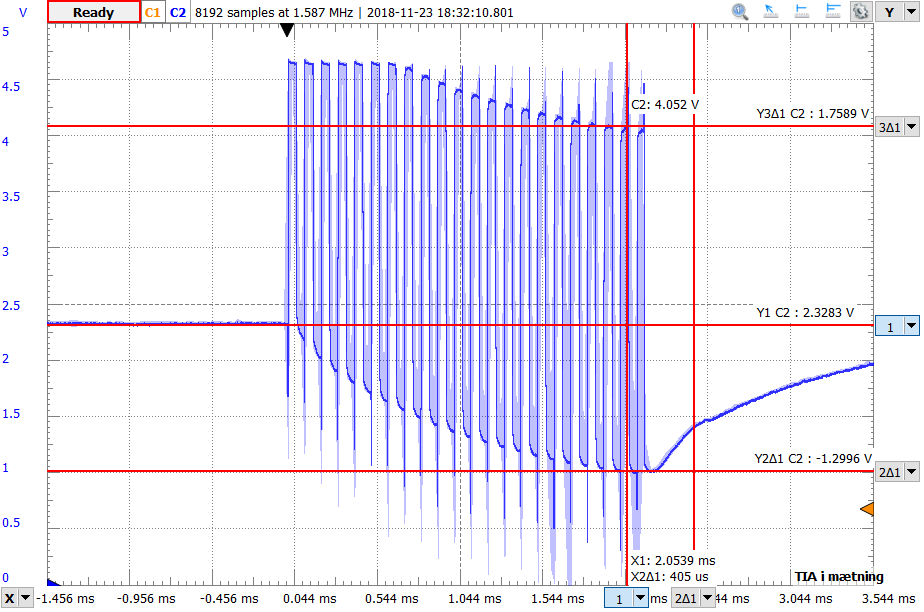
\includegraphics[width=0.9\textwidth]{HardwareDesign/CupSensor/graphics/TIA_saturation.png}
    \caption{Eksempel på en måling hvor TIA'en er gået i mætning.}
    \label{fig:TIA_saturation}
\end{figure}
\paragraph{Udnyttelse af ADC'en område}
Som det ses på \ref{fig:TIA_saturation} så går TIA'en i mætning i starten af læsningen af en sensor. Så selvom den ikke går i mætning i slutningen skal der være en relativ lav forstærkning for at det undgås at den går i mætning i starten. Den maksimale peak-peak værdi (i slustningen af en måling) er målt til kun $2172\si{mV}$. Dette er ikke helt optimalt da hele ADC'ens område er 0V til 5V. ADC'en skal have et område fra 0V til 5V, da det ses på \ref{fig:TIA_saturation}, at spændingen kan komme højere om end den endelige peak-peak værdi. Derudover skal ADC'en have et differentiabel input da signalet er et AC signal med reference til 2.5V (eller deromkring). Men udgangen er grundet mixerfunktionaliteten kun et positivt DC signal, så det maksimale der kan måles er kun $\frac{2172\si{mV}}{2} = 1086\si{mV}$ Det samlede område af ADC'en der benyttes er derfor kun $\frac{1086\si{mV}}{5\si{V}} = 22\%$. Dette er ikke ikke helt omtimalt, da der ikke skal måles fx. en mængde af øl som der er i koppen, men kun tre tilstande: ikke en kop, en kop og ramt, derfor er det ikke så stort et problem.
}

\subsubsection{Stabilitet}

Da fotodioderne har en kondensator og de er på indgangen af en operationsforsærker er det vigtig at bestemme om systemet er stabilt. Der er en kondensator C1 (også omtalt $C_{coupling}$) i serie med kondensatorne i fotodioderne. Den samlede kapacitet for de 24 fotodioder blev tidligere bestemt til at være $C_{C_{total}} = 264\si{pF}$. Da $C_{C_{total}} << C1$, kan C1 ignoreres. Kapaciteten på indgangen er derfor $$C_{C_{total}} = 264\si{pF}$$. 
Kredsløb 4 i øvesle 4 i MSE, benytter et tilsvarende kredsløb som det kan ses på figur \ref{fig:MSE_4_kreds_4}

\begin{figure}
    \centering
    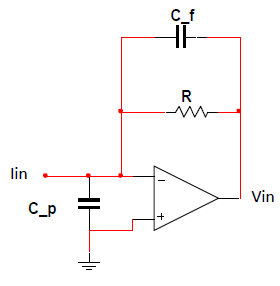
\includegraphics[width=0.7\textwidth]{HardwareDesign/CupSensor/graphics/MSE_EXC_4_opg_4.png}
    \caption{Kredsløb 4 fra øvelse 4 i MSE}
    \label{fig:MSE_4_kreds_4}
\end{figure}

I MSE øvelsen blev det bestemt at systemet er stabilt, i dette tilfælde kritisk dæmpet, når $$C_p=\frac{1}{4\cdot \omega_G \cdot R} - \frac{1}{2}\left( 1 - \frac{1}{2}\omega_G R C_f \right)C_f$$
hvor $\omega_G$ er vinkelfrekvensen for GBW. I tilfældet med sensor kredsløbet kan det overføres til
$$C_p = \frac{1}{4\cdot 2\pi 1\si{MHz} \cdot 80\si{k\Omega}} - \frac{1}{2}\left( 1 - \frac{1}{2} 2\pi 1\si{MHz} \cdot 80\si{k\Omega} 4.6\si{pF} \right)4.6\si{pF} = 0.856\si{pF}$$
Systemet er derfor underdæmpet.

\subsubsection{Støj}
Der er ingen støjspecifikationer for TIA'en så der medtages kun modstandene og fotodiode i beregningerne. 
Først beregnes støjtæthederne på for modstandene.
For modstanden R1
$$i_{nR1} = \sqrt{\frac{4kT}{R_1}} = \sqrt{
\frac{
4\cdot 1.381 \cdot 10^{-23} \cdot \si{
    \frac{V^2}{Hz \cdot \Omega \cdot K}
    }
\cdot 300 \si{K}}{10\si{k\Omega}} } = 1.3 \si{\frac{pA}{\sqrt{Hz}}}$$

For TIA'ens feedback modstand
$$e_{nRf} = \sqrt{4kR_fT} = \sqrt{4\cdot 1.381 \cdot 10^{-23} \cdot  \si{\frac{V^2}{\si{Hz \cdot \Omega \cdot K}}} \cdot 80\si{k\Omega} \cdot 300 \si{K}} = 36.4 \si{\frac{nV}{\sqrt{Hz}}}$$

Herefter beregnes støjtæthederne på udgangen af TIA'en
$$e_{noR1} = i_{nR1} \cdot R_f =1.3 \si{\frac{pA}{\sqrt{Hz}}} \cdot 80\si{k\Omega} = 102 \si{\frac{nV}{\sqrt{Hz}}}$$
$$e_{noRf} = e_{nRf} = 36.4 \si{\frac{nV}{\sqrt{Hz}}}$$

Støjen fra fotodioden antages at være udelukkende shotnoise.
$$i_n = \sqrt{2qI_0}$$
$q = 1.6\cdot 10^{-19} \si{C}$
Det måles at 4 fotodioder udendørs generere en spænding over R1 på $466\si{mV}$. Dette vil for 6 sensorer være $2.8\si{V}$ hvilket svarer til en strøm på $I_0 = \frac{2.8\si{V}}{10\si{k\Omega}} = 280\si{\mu A}$
$$i_n = \sqrt{2 \cdot 1.6\cdot 10^{-19} \si{C} \cdot 280\si{\mu A}} = 9.5 \si{\frac{pA}{\sqrt{Hz}}}$$
$$e_{iout} = R_f \cdot i_n = 80\si{k\Omega} \cdot 9.5 \si{\frac{pA}{\sqrt{Hz}}} = 757 \si{\frac{nV}{\sqrt{Hz}}}$$
 
$$e_{ntot} = \sqrt{e_{nR1}^2 + e_{nRf}^2 + e_{iout}^2} = 765\si{\frac{nV}{\sqrt{Hz}}}$$


$$E_{ntot} = e_{ntot}\cdot \sqrt{BW_n} = 765\si{\frac{nV}{\sqrt{Hz}}}\cdot \sqrt{4\si{kHz}\cdot 2 \cdot \frac{\pi}{2\cdot4}} = 43 \si{\mu V}$$
\subsubsection{Offset}
Det er tidligere blevet vist at et offset i fotodioden ikke vil have nogen indflydelse grundet RC ledet. 
$I_{bias}$ og $I_{ioff}$ er ikke specificeret for TIA'en, men $V_{ioff} = 10mV$ 
$$|V_{TIA\_off}|= 10\si{mV}$$
$$|V_{ADC\_off}| = 0.2\si{mV}$$
I værste tilfælde vil det totale offset være:
$$|V_{tot\_off}| = |V_{TIA\_off}|+|V_{ADC}| = 10.2$$

Dette er ikke så meget relativt til et maksimalt signal på over 1000mV

\subsection{Konklusion}
Der kan på baggrund af analysen konkluderes at der er designet en tilstrækkelig god sensor. 
\end{document}